\documentclass[11pt]{article}
\usepackage[letterpaper,textwidth=5.8in,textheight=8.9in]{geometry}
\usepackage{amsmath,amssymb,graphicx,booktabs,array,tabularx,multirow}
\usepackage[numbers,sort&compress]{natbib}
\usepackage[hidelinks]{hyperref}
\usepackage{microtype}
\usepackage{xcolor}
\usepackage[font=small,labelfont=bf]{caption}
\usepackage[section]{placeins}  % keep each section's floats inside the section
\renewcommand{\topfraction}{0.92}
\renewcommand{\bottomfraction}{0.8}
\renewcommand{\textfraction}{0.06}
\renewcommand{\floatpagefraction}{0.8}
\setcounter{topnumber}{3}
\setcounter{bottomnumber}{2}
\setcounter{totalnumber}{4}
\usepackage{tikz}
\usetikzlibrary{positioning,fit,backgrounds,arrows.meta,calc}
\setlength{\emergencystretch}{2em}
\newcommand{\figpath}{../figures}
% Generated by docs/figures/pusht_numbers.py from docs/results/pusht/. Do not edit by hand.
\newcommand{\PTactMs}{1.8}
\newcommand{\PTbaseCf}{0.0295}
\newcommand{\PTbaseCfBlock}{0.0344}
\newcommand{\PTbaseCfBlockRatio}{1.36}
\newcommand{\PTbaseCfSd}{0.0046}
\newcommand{\PTbaseCopyFifteen}{0.7772}
\newcommand{\PTbaseCopyOne}{0.0368}
\newcommand{\PTbaseCopyRatio}{44}
\newcommand{\PTbaseFactBlock}{0.0162}
\newcommand{\PTbaseGap}{10.2}
\newcommand{\PTbaseImgCopyFifteen}{0.00305}
\newcommand{\PTbaseImgCopyOne}{0.00041}
\newcommand{\PTbaseImgFifteen}{0.00145}
\newcommand{\PTbaseImgOne}{0.00098}
\newcommand{\PTbaseNoop}{0.364}
\newcommand{\PTbaseNoopBlock}{0.0253}
\newcommand{\PTbaseParamsDecoder}{375,811}
\newcommand{\PTbaseParamsHead}{16,770}
\newcommand{\PTbaseParamsNodecM}{0.37}
\newcommand{\PTbaseParamsVla}{238,802}
\newcommand{\PTbaseParamsVlaM}{0.24}
\newcommand{\PTbaseParamsWam}{748,125}
\newcommand{\PTbaseParamsWamM}{0.75}
\newcommand{\PTbasePlan}{37.0}
\newcommand{\PTbasePlanSd}{5.6}
\newcommand{\PTbasePlanSucc}{0}
\newcommand{\PTbaseRtwoFifteen}{0.979}
\newcommand{\PTbaseStateFifteen}{0.0178}
\newcommand{\PTbaseStateFifteenSd}{0.0019}
\newcommand{\PTbaseStateOne}{0.0018}
\newcommand{\PTbaseVla}{24.2}
\newcommand{\PTbaseVlaSd}{6.1}
\newcommand{\PTbaseVlaSucc}{0}
\newcommand{\PTbaseWam}{14.0}
\newcommand{\PTbaseWamSd}{3.2}
\newcommand{\PTbaseWamSucc}{0}
\newcommand{\PTbranchRestartCf}{0.0074}
\newcommand{\PTbranchRestartCfBlock}{0.0104}
\newcommand{\PTbranchRestartCfBlockRatio}{0.41}
\newcommand{\PTbranchRestartCfSd}{0.0012}
\newcommand{\PTbranchRestartCopyFifteen}{0.4973}
\newcommand{\PTbranchRestartCopyOne}{0.0176}
\newcommand{\PTbranchRestartEpochsCf}{0.0038}
\newcommand{\PTbranchRestartEpochsCfBlock}{0.0062}
\newcommand{\PTbranchRestartEpochsCfBlockRatio}{0.24}
\newcommand{\PTbranchRestartEpochsCfSd}{0.0007}
\newcommand{\PTbranchRestartEpochsCopyFifteen}{0.4973}
\newcommand{\PTbranchRestartEpochsCopyOne}{0.0176}
\newcommand{\PTbranchRestartEpochsFactBlock}{0.0070}
\newcommand{\PTbranchRestartEpochsGap}{23.2}
\newcommand{\PTbranchRestartEpochsImgCopyFifteen}{0.00305}
\newcommand{\PTbranchRestartEpochsImgCopyOne}{0.00041}
\newcommand{\PTbranchRestartEpochsImgFifteen}{0.00096}
\newcommand{\PTbranchRestartEpochsImgOne}{0.00057}
\newcommand{\PTbranchRestartEpochsNoop}{0.180}
\newcommand{\PTbranchRestartEpochsNoopBlock}{0.0253}
\newcommand{\PTbranchRestartEpochsParamsDecoder}{375,811}
\newcommand{\PTbranchRestartEpochsParamsHead}{18,576}
\newcommand{\PTbranchRestartEpochsParamsNodecM}{0.37}
\newcommand{\PTbranchRestartEpochsParamsVla}{240,608}
\newcommand{\PTbranchRestartEpochsParamsVlaM}{0.24}
\newcommand{\PTbranchRestartEpochsParamsWam}{749,931}
\newcommand{\PTbranchRestartEpochsParamsWamM}{0.75}
\newcommand{\PTbranchRestartEpochsPlan}{56.8}
\newcommand{\PTbranchRestartEpochsPlanExpected}{23.5}
\newcommand{\PTbranchRestartEpochsPlanPlanErr}{32.5}
\newcommand{\PTbranchRestartEpochsPlanReal}{\ensuremath{-}0.1}
\newcommand{\PTbranchRestartEpochsPlanSd}{6.3}
\newcommand{\PTbranchRestartEpochsPlanSucc}{77}
\newcommand{\PTbranchRestartEpochsPlanWarm}{37.4}
\newcommand{\PTbranchRestartEpochsPlanWarmExpected}{30.2}
\newcommand{\PTbranchRestartEpochsPlanWarmPlanErr}{40.2}
\newcommand{\PTbranchRestartEpochsPlanWarmReal}{\ensuremath{-}1.5}
\newcommand{\PTbranchRestartEpochsPlanWarmSd}{9.5}
\newcommand{\PTbranchRestartEpochsPlanWarmSucc}{11}
\newcommand{\PTbranchRestartEpochsRtwoFifteen}{0.990}
\newcommand{\PTbranchRestartEpochsStateFifteen}{0.0083}
\newcommand{\PTbranchRestartEpochsStateFifteenSd}{0.0013}
\newcommand{\PTbranchRestartEpochsStateOne}{0.0006}
\newcommand{\PTbranchRestartEpochsVla}{63.5}
\newcommand{\PTbranchRestartEpochsVlaSd}{9.0}
\newcommand{\PTbranchRestartEpochsVlaSucc}{57}
\newcommand{\PTbranchRestartEpochsWam}{40.3}
\newcommand{\PTbranchRestartEpochsWamSd}{2.6}
\newcommand{\PTbranchRestartEpochsWamSucc}{7}
\newcommand{\PTbranchRestartFactBlock}{0.0106}
\newcommand{\PTbranchRestartGap}{12.8}
\newcommand{\PTbranchRestartImgCopyFifteen}{0.00305}
\newcommand{\PTbranchRestartImgCopyOne}{0.00041}
\newcommand{\PTbranchRestartImgFifteen}{0.00127}
\newcommand{\PTbranchRestartImgOne}{0.00080}
\newcommand{\PTbranchRestartNoop}{0.180}
\newcommand{\PTbranchRestartNoopBlock}{0.0253}
\newcommand{\PTbranchRestartParamsDecoder}{375,811}
\newcommand{\PTbranchRestartParamsHead}{18,576}
\newcommand{\PTbranchRestartParamsNodecM}{0.37}
\newcommand{\PTbranchRestartParamsVla}{240,608}
\newcommand{\PTbranchRestartParamsVlaM}{0.24}
\newcommand{\PTbranchRestartParamsWam}{749,931}
\newcommand{\PTbranchRestartParamsWamM}{0.75}
\newcommand{\PTbranchRestartPlan}{51.5}
\newcommand{\PTbranchRestartPlanExpected}{21.7}
\newcommand{\PTbranchRestartPlanPlanErr}{31.9}
\newcommand{\PTbranchRestartPlanReal}{\ensuremath{-}1.0}
\newcommand{\PTbranchRestartPlanSd}{1.4}
\newcommand{\PTbranchRestartPlanSucc}{32}
\newcommand{\PTbranchRestartPlanWarm}{43.6}
\newcommand{\PTbranchRestartPlanWarmExpected}{24.5}
\newcommand{\PTbranchRestartPlanWarmPlanErr}{31.5}
\newcommand{\PTbranchRestartPlanWarmReal}{0.3}
\newcommand{\PTbranchRestartPlanWarmSd}{2.9}
\newcommand{\PTbranchRestartPlanWarmSucc}{17}
\newcommand{\PTbranchRestartRtwoFifteen}{0.983}
\newcommand{\PTbranchRestartStateFifteen}{0.0138}
\newcommand{\PTbranchRestartStateFifteenSd}{0.0040}
\newcommand{\PTbranchRestartStateOne}{0.0014}
\newcommand{\PTbranchRestartVla}{37.6}
\newcommand{\PTbranchRestartVlaSd}{8.1}
\newcommand{\PTbranchRestartVlaSucc}{8}
\newcommand{\PTbranchRestartWam}{24.7}
\newcommand{\PTbranchRestartWamSd}{2.0}
\newcommand{\PTbranchRestartWamSucc}{2}
\newcommand{\PTbudgetCf}{0.0318}
\newcommand{\PTbudgetCfBlock}{0.0350}
\newcommand{\PTbudgetCfBlockRatio}{1.38}
\newcommand{\PTbudgetCfSd}{0.0014}
\newcommand{\PTbudgetCopyFifteen}{0.7772}
\newcommand{\PTbudgetCopyOne}{0.0368}
\newcommand{\PTbudgetFactBlock}{0.0151}
\newcommand{\PTbudgetGap}{6.9}
\newcommand{\PTbudgetImgCopyFifteen}{0.00305}
\newcommand{\PTbudgetImgCopyOne}{0.00041}
\newcommand{\PTbudgetImgFifteen}{0.00142}
\newcommand{\PTbudgetImgOne}{0.00099}
\newcommand{\PTbudgetNoop}{0.364}
\newcommand{\PTbudgetNoopBlock}{0.0253}
\newcommand{\PTbudgetPlan}{33.8}
\newcommand{\PTbudgetPlanCem}{18.2}
\newcommand{\PTbudgetPlanCemExpected}{82.1}
\newcommand{\PTbudgetPlanCemPlanErr}{103.7}
\newcommand{\PTbudgetPlanCemReal}{\ensuremath{-}1.9}
\newcommand{\PTbudgetPlanCemSd}{0.6}
\newcommand{\PTbudgetPlanCemSucc}{0}
\newcommand{\PTbudgetPlanExpected}{33.3}
\newcommand{\PTbudgetPlanNoprior}{9.6}
\newcommand{\PTbudgetPlanNopriorExpected}{85.7}
\newcommand{\PTbudgetPlanNopriorPlanErr}{104.5}
\newcommand{\PTbudgetPlanNopriorReal}{\ensuremath{-}0.1}
\newcommand{\PTbudgetPlanNopriorSd}{1.2}
\newcommand{\PTbudgetPlanNopriorSucc}{0}
\newcommand{\PTbudgetPlanPlanErr}{47.6}
\newcommand{\PTbudgetPlanReal}{\ensuremath{-}1.5}
\newcommand{\PTbudgetPlanSd}{3.6}
\newcommand{\PTbudgetPlanSucc}{0}
\newcommand{\PTbudgetPlanWide}{23.0}
\newcommand{\PTbudgetPlanWideExpected}{56.1}
\newcommand{\PTbudgetPlanWidePlanErr}{76.6}
\newcommand{\PTbudgetPlanWideReal}{\ensuremath{-}1.3}
\newcommand{\PTbudgetPlanWideSd}{2.3}
\newcommand{\PTbudgetPlanWideSucc}{0}
\newcommand{\PTbudgetRtwoFifteen}{0.981}
\newcommand{\PTbudgetStateFifteen}{0.0161}
\newcommand{\PTbudgetStateFifteenSd}{0.0039}
\newcommand{\PTbudgetStateOne}{0.0022}
\newcommand{\PTbudgetVla}{21.5}
\newcommand{\PTbudgetVlaSd}{6.5}
\newcommand{\PTbudgetVlaSucc}{0}
\newcommand{\PTbudgetWam}{14.6}
\newcommand{\PTbudgetWamSd}{3.7}
\newcommand{\PTbudgetWamSucc}{0}
\newcommand{\PTchunkBranchCf}{0.0085}
\newcommand{\PTchunkBranchCfBlock}{0.0114}
\newcommand{\PTchunkBranchCfBlockRatio}{0.45}
\newcommand{\PTchunkBranchCfSd}{0.0020}
\newcommand{\PTchunkBranchCopyFifteen}{0.4973}
\newcommand{\PTchunkBranchCopyOne}{0.0176}
\newcommand{\PTchunkBranchFactBlock}{0.0138}
\newcommand{\PTchunkBranchGap}{12.0}
\newcommand{\PTchunkBranchImgCopyFifteen}{0.00305}
\newcommand{\PTchunkBranchImgCopyOne}{0.00041}
\newcommand{\PTchunkBranchImgFifteen}{0.00137}
\newcommand{\PTchunkBranchImgOne}{0.00077}
\newcommand{\PTchunkBranchNoop}{0.180}
\newcommand{\PTchunkBranchNoopBlock}{0.0253}
\newcommand{\PTchunkBranchParamsDecoder}{375,811}
\newcommand{\PTchunkBranchParamsHead}{18,576}
\newcommand{\PTchunkBranchParamsNodecM}{0.37}
\newcommand{\PTchunkBranchParamsVla}{240,608}
\newcommand{\PTchunkBranchParamsVlaM}{0.24}
\newcommand{\PTchunkBranchParamsWam}{749,931}
\newcommand{\PTchunkBranchParamsWamM}{0.75}
\newcommand{\PTchunkBranchPlan}{44.9}
\newcommand{\PTchunkBranchPlanSd}{7.2}
\newcommand{\PTchunkBranchPlanSucc}{13}
\newcommand{\PTchunkBranchRtwoFifteen}{0.980}
\newcommand{\PTchunkBranchStateFifteen}{0.0167}
\newcommand{\PTchunkBranchStateFifteenSd}{0.0026}
\newcommand{\PTchunkBranchStateOne}{0.0017}
\newcommand{\PTchunkBranchVla}{35.8}
\newcommand{\PTchunkBranchVlaSd}{9.9}
\newcommand{\PTchunkBranchVlaSucc}{7}
\newcommand{\PTchunkBranchWam}{23.8}
\newcommand{\PTchunkBranchWamSd}{3.9}
\newcommand{\PTchunkBranchWamSucc}{0}
\newcommand{\PTchunkCf}{0.0265}
\newcommand{\PTchunkCfBlock}{0.0331}
\newcommand{\PTchunkCfBlockRatio}{1.31}
\newcommand{\PTchunkCfSd}{0.0035}
\newcommand{\PTchunkCnnCf}{0.0242}
\newcommand{\PTchunkCnnCfBlock}{0.0290}
\newcommand{\PTchunkCnnCfBlockRatio}{1.14}
\newcommand{\PTchunkCnnCfSd}{0.0036}
\newcommand{\PTchunkCnnCopyFifteen}{0.7772}
\newcommand{\PTchunkCnnCopyOne}{0.0368}
\newcommand{\PTchunkCnnFactBlock}{0.0159}
\newcommand{\PTchunkCnnGap}{26.2}
\newcommand{\PTchunkCnnImgCopyFifteen}{0.00305}
\newcommand{\PTchunkCnnImgCopyOne}{0.00041}
\newcommand{\PTchunkCnnImgFifteen}{0.00137}
\newcommand{\PTchunkCnnImgOne}{0.00101}
\newcommand{\PTchunkCnnNoop}{0.364}
\newcommand{\PTchunkCnnNoopBlock}{0.0253}
\newcommand{\PTchunkCnnParamsDecoder}{375,811}
\newcommand{\PTchunkCnnParamsHead}{18,576}
\newcommand{\PTchunkCnnParamsNodecM}{0.41}
\newcommand{\PTchunkCnnParamsVla}{280,592}
\newcommand{\PTchunkCnnParamsVlaM}{0.28}
\newcommand{\PTchunkCnnParamsWam}{789,915}
\newcommand{\PTchunkCnnParamsWamM}{0.79}
\newcommand{\PTchunkCnnPlan}{43.6}
\newcommand{\PTchunkCnnPlanSd}{1.2}
\newcommand{\PTchunkCnnPlanSucc}{1}
\newcommand{\PTchunkCnnRtwoFifteen}{0.979}
\newcommand{\PTchunkCnnStateFifteen}{0.0180}
\newcommand{\PTchunkCnnStateFifteenSd}{0.0056}
\newcommand{\PTchunkCnnStateOne}{0.0023}
\newcommand{\PTchunkCnnVla}{44.7}
\newcommand{\PTchunkCnnVlaSd}{9.0}
\newcommand{\PTchunkCnnVlaSucc}{7}
\newcommand{\PTchunkCnnWam}{18.4}
\newcommand{\PTchunkCnnWamSd}{4.5}
\newcommand{\PTchunkCnnWamSucc}{0}
\newcommand{\PTchunkCopyFifteen}{0.7772}
\newcommand{\PTchunkCopyOne}{0.0368}
\newcommand{\PTchunkEnsembleCf}{0.0270}
\newcommand{\PTchunkEnsembleCfBlock}{0.0314}
\newcommand{\PTchunkEnsembleCfBlockRatio}{1.25}
\newcommand{\PTchunkEnsembleCfSd}{0.0027}
\newcommand{\PTchunkEnsembleCopyFifteen}{0.7772}
\newcommand{\PTchunkEnsembleCopyOne}{0.0368}
\newcommand{\PTchunkEnsembleFactBlock}{0.0159}
\newcommand{\PTchunkEnsembleGap}{17.0}
\newcommand{\PTchunkEnsembleImgCopyFifteen}{0.00305}
\newcommand{\PTchunkEnsembleImgCopyOne}{0.00041}
\newcommand{\PTchunkEnsembleImgFifteen}{0.00141}
\newcommand{\PTchunkEnsembleImgOne}{0.00101}
\newcommand{\PTchunkEnsembleNoop}{0.364}
\newcommand{\PTchunkEnsembleNoopBlock}{0.0253}
\newcommand{\PTchunkEnsembleParamsDecoder}{375,811}
\newcommand{\PTchunkEnsembleParamsHead}{18,576}
\newcommand{\PTchunkEnsembleParamsNodecM}{0.37}
\newcommand{\PTchunkEnsembleParamsVla}{240,608}
\newcommand{\PTchunkEnsembleParamsVlaM}{0.24}
\newcommand{\PTchunkEnsembleParamsWam}{749,931}
\newcommand{\PTchunkEnsembleParamsWamM}{0.75}
\newcommand{\PTchunkEnsemblePlan}{36.5}
\newcommand{\PTchunkEnsemblePlanSd}{2.1}
\newcommand{\PTchunkEnsemblePlanSucc}{0}
\newcommand{\PTchunkEnsembleRtwoFifteen}{0.977}
\newcommand{\PTchunkEnsembleStateFifteen}{0.0192}
\newcommand{\PTchunkEnsembleStateFifteenSd}{0.0037}
\newcommand{\PTchunkEnsembleStateOne}{0.0025}
\newcommand{\PTchunkEnsembleVla}{39.0}
\newcommand{\PTchunkEnsembleVlaSd}{6.6}
\newcommand{\PTchunkEnsembleVlaSucc}{3}
\newcommand{\PTchunkEnsembleWam}{22.0}
\newcommand{\PTchunkEnsembleWamSd}{1.4}
\newcommand{\PTchunkEnsembleWamSucc}{0}
\newcommand{\PTchunkEpochsCf}{0.0165}
\newcommand{\PTchunkEpochsCfBlock}{0.0264}
\newcommand{\PTchunkEpochsCfBlockRatio}{1.04}
\newcommand{\PTchunkEpochsCfSd}{0.0019}
\newcommand{\PTchunkEpochsCopyFifteen}{0.7772}
\newcommand{\PTchunkEpochsCopyOne}{0.0368}
\newcommand{\PTchunkEpochsFactBlock}{0.0109}
\newcommand{\PTchunkEpochsGap}{21.6}
\newcommand{\PTchunkEpochsImgCopyFifteen}{0.00305}
\newcommand{\PTchunkEpochsImgCopyOne}{0.00041}
\newcommand{\PTchunkEpochsImgFifteen}{0.00112}
\newcommand{\PTchunkEpochsImgOne}{0.00076}
\newcommand{\PTchunkEpochsNoop}{0.364}
\newcommand{\PTchunkEpochsNoopBlock}{0.0253}
\newcommand{\PTchunkEpochsParamsDecoder}{375,811}
\newcommand{\PTchunkEpochsParamsHead}{18,576}
\newcommand{\PTchunkEpochsParamsNodecM}{0.37}
\newcommand{\PTchunkEpochsParamsVla}{240,608}
\newcommand{\PTchunkEpochsParamsVlaM}{0.24}
\newcommand{\PTchunkEpochsParamsWam}{749,931}
\newcommand{\PTchunkEpochsParamsWamM}{0.75}
\newcommand{\PTchunkEpochsPlan}{20.2}
\newcommand{\PTchunkEpochsPlanSd}{0.8}
\newcommand{\PTchunkEpochsPlanSucc}{0}
\newcommand{\PTchunkEpochsRtwoFifteen}{0.987}
\newcommand{\PTchunkEpochsStateFifteen}{0.0112}
\newcommand{\PTchunkEpochsStateFifteenSd}{0.0036}
\newcommand{\PTchunkEpochsStateOne}{0.0011}
\newcommand{\PTchunkEpochsVla}{68.0}
\newcommand{\PTchunkEpochsVlaSd}{2.3}
\newcommand{\PTchunkEpochsVlaSucc}{62}
\newcommand{\PTchunkEpochsWam}{46.4}
\newcommand{\PTchunkEpochsWamSd}{3.1}
\newcommand{\PTchunkEpochsWamSucc}{9}
\newcommand{\PTchunkFactBlock}{0.0174}
\newcommand{\PTchunkGap}{16.7}
\newcommand{\PTchunkImgCopyFifteen}{0.00305}
\newcommand{\PTchunkImgCopyOne}{0.00041}
\newcommand{\PTchunkImgFifteen}{0.00140}
\newcommand{\PTchunkImgOne}{0.00096}
\newcommand{\PTchunkNarrowCf}{0.0237}
\newcommand{\PTchunkNarrowCfBlock}{0.0302}
\newcommand{\PTchunkNarrowCfBlockRatio}{1.20}
\newcommand{\PTchunkNarrowCfSd}{0.0014}
\newcommand{\PTchunkNarrowCopyFifteen}{0.7772}
\newcommand{\PTchunkNarrowCopyOne}{0.0368}
\newcommand{\PTchunkNarrowFactBlock}{0.0155}
\newcommand{\PTchunkNarrowGap}{15.0}
\newcommand{\PTchunkNarrowImgCopyFifteen}{0.00305}
\newcommand{\PTchunkNarrowImgCopyOne}{0.00041}
\newcommand{\PTchunkNarrowImgFifteen}{0.00141}
\newcommand{\PTchunkNarrowImgOne}{0.00103}
\newcommand{\PTchunkNarrowNoop}{0.364}
\newcommand{\PTchunkNarrowNoopBlock}{0.0253}
\newcommand{\PTchunkNarrowParamsDecoder}{244,739}
\newcommand{\PTchunkNarrowParamsHead}{5,200}
\newcommand{\PTchunkNarrowParamsNodecM}{0.22}
\newcommand{\PTchunkNarrowParamsVla}{117,536}
\newcommand{\PTchunkNarrowParamsVlaM}{0.12}
\newcommand{\PTchunkNarrowParamsWam}{462,315}
\newcommand{\PTchunkNarrowParamsWamM}{0.46}
\newcommand{\PTchunkNarrowPlan}{36.3}
\newcommand{\PTchunkNarrowPlanSd}{2.7}
\newcommand{\PTchunkNarrowPlanSucc}{0}
\newcommand{\PTchunkNarrowRtwoFifteen}{0.980}
\newcommand{\PTchunkNarrowStateFifteen}{0.0168}
\newcommand{\PTchunkNarrowStateFifteenSd}{0.0048}
\newcommand{\PTchunkNarrowStateOne}{0.0019}
\newcommand{\PTchunkNarrowVla}{32.2}
\newcommand{\PTchunkNarrowVlaSd}{4.2}
\newcommand{\PTchunkNarrowVlaSucc}{1}
\newcommand{\PTchunkNarrowWam}{17.2}
\newcommand{\PTchunkNarrowWamSd}{2.3}
\newcommand{\PTchunkNarrowWamSucc}{0}
\newcommand{\PTchunkNodecCf}{0.0246}
\newcommand{\PTchunkNodecCfBlock}{0.0287}
\newcommand{\PTchunkNodecCfBlockRatio}{1.14}
\newcommand{\PTchunkNodecCfSd}{0.0026}
\newcommand{\PTchunkNodecCopyFifteen}{0.7772}
\newcommand{\PTchunkNodecCopyOne}{0.0368}
\newcommand{\PTchunkNodecFactBlock}{0.0182}
\newcommand{\PTchunkNodecGap}{14.2}
\newcommand{\PTchunkNodecNoop}{0.364}
\newcommand{\PTchunkNodecNoopBlock}{0.0253}
\newcommand{\PTchunkNodecParamsHead}{18,576}
\newcommand{\PTchunkNodecParamsVla}{240,608}
\newcommand{\PTchunkNodecParamsVlaM}{0.24}
\newcommand{\PTchunkNodecParamsWam}{374,120}
\newcommand{\PTchunkNodecParamsWamM}{0.37}
\newcommand{\PTchunkNodecPlan}{38.0}
\newcommand{\PTchunkNodecPlanSd}{3.4}
\newcommand{\PTchunkNodecPlanSucc}{1}
\newcommand{\PTchunkNodecRtwoFifteen}{0.976}
\newcommand{\PTchunkNodecStateFifteen}{0.0201}
\newcommand{\PTchunkNodecStateFifteenSd}{0.0047}
\newcommand{\PTchunkNodecStateOne}{0.0027}
\newcommand{\PTchunkNodecVla}{37.3}
\newcommand{\PTchunkNodecVlaSd}{12.0}
\newcommand{\PTchunkNodecVlaSucc}{3}
\newcommand{\PTchunkNodecWam}{23.1}
\newcommand{\PTchunkNodecWamSd}{4.3}
\newcommand{\PTchunkNodecWamSucc}{1}
\newcommand{\PTchunkNoop}{0.364}
\newcommand{\PTchunkNoopBlock}{0.0253}
\newcommand{\PTchunkParamsDecoder}{375,811}
\newcommand{\PTchunkParamsHead}{18,576}
\newcommand{\PTchunkParamsNodecM}{0.37}
\newcommand{\PTchunkParamsVla}{240,608}
\newcommand{\PTchunkParamsVlaM}{0.24}
\newcommand{\PTchunkParamsWam}{749,931}
\newcommand{\PTchunkParamsWamM}{0.75}
\newcommand{\PTchunkPlan}{39.2}
\newcommand{\PTchunkPlanSd}{8.5}
\newcommand{\PTchunkPlanSucc}{1}
\newcommand{\PTchunkRestartCf}{0.0263}
\newcommand{\PTchunkRestartCfBlock}{0.0297}
\newcommand{\PTchunkRestartCfBlockRatio}{1.18}
\newcommand{\PTchunkRestartCfSd}{0.0018}
\newcommand{\PTchunkRestartCopyFifteen}{0.7772}
\newcommand{\PTchunkRestartCopyOne}{0.0368}
\newcommand{\PTchunkRestartFactBlock}{0.0157}
\newcommand{\PTchunkRestartGap}{17.6}
\newcommand{\PTchunkRestartImgCopyFifteen}{0.00305}
\newcommand{\PTchunkRestartImgCopyOne}{0.00041}
\newcommand{\PTchunkRestartImgFifteen}{0.00141}
\newcommand{\PTchunkRestartImgOne}{0.00101}
\newcommand{\PTchunkRestartNoop}{0.364}
\newcommand{\PTchunkRestartNoopBlock}{0.0253}
\newcommand{\PTchunkRestartParamsDecoder}{375,811}
\newcommand{\PTchunkRestartParamsHead}{18,576}
\newcommand{\PTchunkRestartParamsNodecM}{0.37}
\newcommand{\PTchunkRestartParamsVla}{240,608}
\newcommand{\PTchunkRestartParamsVlaM}{0.24}
\newcommand{\PTchunkRestartParamsWam}{749,931}
\newcommand{\PTchunkRestartParamsWamM}{0.75}
\newcommand{\PTchunkRestartPlan}{44.0}
\newcommand{\PTchunkRestartPlanExpected}{23.4}
\newcommand{\PTchunkRestartPlanPlanErr}{37.2}
\newcommand{\PTchunkRestartPlanReal}{\ensuremath{-}0.8}
\newcommand{\PTchunkRestartPlanSd}{10.6}
\newcommand{\PTchunkRestartPlanSucc}{4}
\newcommand{\PTchunkRestartPlanWarm}{42.8}
\newcommand{\PTchunkRestartPlanWarmExpected}{33.6}
\newcommand{\PTchunkRestartPlanWarmPlanErr}{48.7}
\newcommand{\PTchunkRestartPlanWarmReal}{\ensuremath{-}0.8}
\newcommand{\PTchunkRestartPlanWarmSd}{8.5}
\newcommand{\PTchunkRestartPlanWarmSucc}{0}
\newcommand{\PTchunkRestartRtwoFifteen}{0.977}
\newcommand{\PTchunkRestartStateFifteen}{0.0197}
\newcommand{\PTchunkRestartStateFifteenSd}{0.0042}
\newcommand{\PTchunkRestartStateOne}{0.0024}
\newcommand{\PTchunkRestartVla}{39.2}
\newcommand{\PTchunkRestartVlaSd}{10.0}
\newcommand{\PTchunkRestartVlaSucc}{6}
\newcommand{\PTchunkRestartWam}{21.6}
\newcommand{\PTchunkRestartWamSd}{4.4}
\newcommand{\PTchunkRestartWamSucc}{0}
\newcommand{\PTchunkRtwoFifteen}{0.976}
\newcommand{\PTchunkSixteenCf}{0.0262}
\newcommand{\PTchunkSixteenCfBlock}{0.0330}
\newcommand{\PTchunkSixteenCfBlockRatio}{1.31}
\newcommand{\PTchunkSixteenCfSd}{0.0006}
\newcommand{\PTchunkSixteenCopyFifteen}{0.7772}
\newcommand{\PTchunkSixteenCopyOne}{0.0368}
\newcommand{\PTchunkSixteenFactBlock}{0.0166}
\newcommand{\PTchunkSixteenGap}{14.8}
\newcommand{\PTchunkSixteenImgCopyFifteen}{0.00305}
\newcommand{\PTchunkSixteenImgCopyOne}{0.00041}
\newcommand{\PTchunkSixteenImgFifteen}{0.00146}
\newcommand{\PTchunkSixteenImgOne}{0.00098}
\newcommand{\PTchunkSixteenNoop}{0.364}
\newcommand{\PTchunkSixteenNoopBlock}{0.0253}
\newcommand{\PTchunkSixteenParamsDecoder}{375,811}
\newcommand{\PTchunkSixteenParamsHead}{20,640}
\newcommand{\PTchunkSixteenParamsNodecM}{0.38}
\newcommand{\PTchunkSixteenParamsVla}{242,672}
\newcommand{\PTchunkSixteenParamsVlaM}{0.24}
\newcommand{\PTchunkSixteenParamsWam}{751,995}
\newcommand{\PTchunkSixteenParamsWamM}{0.75}
\newcommand{\PTchunkSixteenPlan}{38.7}
\newcommand{\PTchunkSixteenPlanSd}{3.1}
\newcommand{\PTchunkSixteenPlanSucc}{0}
\newcommand{\PTchunkSixteenRtwoFifteen}{0.977}
\newcommand{\PTchunkSixteenStateFifteen}{0.0185}
\newcommand{\PTchunkSixteenStateFifteenSd}{0.0030}
\newcommand{\PTchunkSixteenStateOne}{0.0023}
\newcommand{\PTchunkSixteenVla}{32.5}
\newcommand{\PTchunkSixteenVlaSd}{4.2}
\newcommand{\PTchunkSixteenVlaSucc}{3}
\newcommand{\PTchunkSixteenWam}{17.7}
\newcommand{\PTchunkSixteenWamSd}{0.5}
\newcommand{\PTchunkSixteenWamSucc}{1}
\newcommand{\PTchunkStateFifteen}{0.0202}
\newcommand{\PTchunkStateFifteenSd}{0.0031}
\newcommand{\PTchunkStateOne}{0.0027}
\newcommand{\PTchunkVla}{40.2}
\newcommand{\PTchunkVlaSd}{8.8}
\newcommand{\PTchunkVlaSucc}{4}
\newcommand{\PTchunkWam}{23.5}
\newcommand{\PTchunkWamSd}{5.8}
\newcommand{\PTchunkWamSucc}{5}
\newcommand{\PTdataBlockErrPninetynine}{0.53}
\newcommand{\PTdataBlockMove}{3.7}
\newcommand{\PTdataClipped}{29}
\newcommand{\PTdataDemoCoverage}{84.8}
\newcommand{\PTdataDemoSuccesses}{0}
\newcommand{\PTdataRender}{0.95}
\newcommand{\PTdfiftyCf}{0.0375}
\newcommand{\PTdfiftyCfBlock}{0.0394}
\newcommand{\PTdfiftyCfBlockRatio}{1.57}
\newcommand{\PTdfiftyCfSd}{0.0048}
\newcommand{\PTdfiftyCopyFifteen}{0.7083}
\newcommand{\PTdfiftyCopyOne}{0.0411}
\newcommand{\PTdfiftyFactBlock}{0.0402}
\newcommand{\PTdfiftyGap}{2.5}
\newcommand{\PTdfiftyImgCopyFifteen}{0.00310}
\newcommand{\PTdfiftyImgCopyOne}{0.00037}
\newcommand{\PTdfiftyImgFifteen}{0.00224}
\newcommand{\PTdfiftyImgOne}{0.00177}
\newcommand{\PTdfiftyNoop}{0.434}
\newcommand{\PTdfiftyNoopBlock}{0.0251}
\newcommand{\PTdfiftyParamsDecoder}{375,811}
\newcommand{\PTdfiftyParamsHead}{16,770}
\newcommand{\PTdfiftyParamsNodecM}{0.37}
\newcommand{\PTdfiftyParamsVla}{238,802}
\newcommand{\PTdfiftyParamsVlaM}{0.24}
\newcommand{\PTdfiftyParamsWam}{748,125}
\newcommand{\PTdfiftyParamsWamM}{0.75}
\newcommand{\PTdfiftyPlan}{19.0}
\newcommand{\PTdfiftyPlanSd}{3.7}
\newcommand{\PTdfiftyPlanSucc}{0}
\newcommand{\PTdfiftyRtwoFifteen}{0.936}
\newcommand{\PTdfiftyStateFifteen}{0.0396}
\newcommand{\PTdfiftyStateFifteenSd}{0.0031}
\newcommand{\PTdfiftyStateOne}{0.0049}
\newcommand{\PTdfiftyVla}{13.6}
\newcommand{\PTdfiftyVlaSd}{2.0}
\newcommand{\PTdfiftyVlaSucc}{0}
\newcommand{\PTdfiftyWam}{11.0}
\newcommand{\PTdfiftyWamSd}{2.8}
\newcommand{\PTdfiftyWamSucc}{0}
\newcommand{\PTdhundredCf}{0.0398}
\newcommand{\PTdhundredCfBlock}{0.0434}
\newcommand{\PTdhundredCfBlockRatio}{1.69}
\newcommand{\PTdhundredCfSd}{0.0010}
\newcommand{\PTdhundredCopyFifteen}{0.6623}
\newcommand{\PTdhundredCopyOne}{0.0427}
\newcommand{\PTdhundredFactBlock}{0.0234}
\newcommand{\PTdhundredGap}{4.0}
\newcommand{\PTdhundredImgCopyFifteen}{0.00312}
\newcommand{\PTdhundredImgCopyOne}{0.00037}
\newcommand{\PTdhundredImgFifteen}{0.00179}
\newcommand{\PTdhundredImgOne}{0.00125}
\newcommand{\PTdhundredNoop}{0.404}
\newcommand{\PTdhundredNoopBlock}{0.0259}
\newcommand{\PTdhundredParamsDecoder}{375,811}
\newcommand{\PTdhundredParamsHead}{16,770}
\newcommand{\PTdhundredParamsNodecM}{0.37}
\newcommand{\PTdhundredParamsVla}{238,802}
\newcommand{\PTdhundredParamsVlaM}{0.24}
\newcommand{\PTdhundredParamsWam}{748,125}
\newcommand{\PTdhundredParamsWamM}{0.75}
\newcommand{\PTdhundredPlan}{24.5}
\newcommand{\PTdhundredPlanSd}{3.3}
\newcommand{\PTdhundredPlanSucc}{0}
\newcommand{\PTdhundredRtwoFifteen}{0.966}
\newcommand{\PTdhundredStateFifteen}{0.0241}
\newcommand{\PTdhundredStateFifteenSd}{0.0036}
\newcommand{\PTdhundredStateOne}{0.0025}
\newcommand{\PTdhundredVla}{16.7}
\newcommand{\PTdhundredVlaSd}{7.3}
\newcommand{\PTdhundredVlaSucc}{0}
\newcommand{\PTdhundredWam}{12.7}
\newcommand{\PTdhundredWamSd}{2.2}
\newcommand{\PTdhundredWamSucc}{0}
\newcommand{\PTdiffCf}{0.0437}
\newcommand{\PTdiffCfBlock}{0.0451}
\newcommand{\PTdiffCfBlockRatio}{1.78}
\newcommand{\PTdiffCfSd}{0.0073}
\newcommand{\PTdiffCopyFifteen}{0.7772}
\newcommand{\PTdiffCopyOne}{0.0368}
\newcommand{\PTdiffFactBlock}{0.0331}
\newcommand{\PTdiffGap}{3.6}
\newcommand{\PTdiffImgCopyFifteen}{0.00305}
\newcommand{\PTdiffImgCopyOne}{0.00041}
\newcommand{\PTdiffImgFifteen}{0.00197}
\newcommand{\PTdiffImgOne}{0.00123}
\newcommand{\PTdiffNoop}{0.364}
\newcommand{\PTdiffNoopBlock}{0.0253}
\newcommand{\PTdiffParamsDecoder}{375,811}
\newcommand{\PTdiffParamsHead}{37,634}
\newcommand{\PTdiffParamsNodecM}{0.39}
\newcommand{\PTdiffParamsVla}{259,666}
\newcommand{\PTdiffParamsVlaM}{0.26}
\newcommand{\PTdiffParamsWam}{768,989}
\newcommand{\PTdiffParamsWamM}{0.77}
\newcommand{\PTdiffPlan}{15.2}
\newcommand{\PTdiffPlanSd}{4.3}
\newcommand{\PTdiffPlanSucc}{0}
\newcommand{\PTdiffRtwoFifteen}{0.951}
\newcommand{\PTdiffStateFifteen}{0.0417}
\newcommand{\PTdiffStateFifteenSd}{0.0114}
\newcommand{\PTdiffStateOne}{0.0050}
\newcommand{\PTdiffVla}{14.2}
\newcommand{\PTdiffVlaSd}{2.8}
\newcommand{\PTdiffVlaSucc}{0}
\newcommand{\PTdiffWam}{10.6}
\newcommand{\PTdiffWamSd}{3.0}
\newcommand{\PTdiffWamSucc}{0}
\newcommand{\PTepochsCf}{0.0147}
\newcommand{\PTepochsCfBlock}{0.0234}
\newcommand{\PTepochsCfBlockRatio}{0.92}
\newcommand{\PTepochsCfSd}{0.0032}
\newcommand{\PTepochsCopyFifteen}{0.7772}
\newcommand{\PTepochsCopyOne}{0.0368}
\newcommand{\PTepochsFactBlock}{0.0070}
\newcommand{\PTepochsGap}{10.0}
\newcommand{\PTepochsImgCopyFifteen}{0.00305}
\newcommand{\PTepochsImgCopyOne}{0.00041}
\newcommand{\PTepochsImgFifteen}{0.00095}
\newcommand{\PTepochsImgOne}{0.00069}
\newcommand{\PTepochsNoop}{0.364}
\newcommand{\PTepochsNoopBlock}{0.0253}
\newcommand{\PTepochsParamsDecoder}{375,811}
\newcommand{\PTepochsParamsHead}{16,770}
\newcommand{\PTepochsParamsNodecM}{0.37}
\newcommand{\PTepochsParamsVla}{238,802}
\newcommand{\PTepochsParamsVlaM}{0.24}
\newcommand{\PTepochsParamsWam}{748,125}
\newcommand{\PTepochsParamsWamM}{0.75}
\newcommand{\PTepochsPlan}{19.3}
\newcommand{\PTepochsPlanSd}{3.6}
\newcommand{\PTepochsPlanSucc}{0}
\newcommand{\PTepochsRtwoFifteen}{0.991}
\newcommand{\PTepochsStateFifteen}{0.0078}
\newcommand{\PTepochsStateFifteenSd}{0.0013}
\newcommand{\PTepochsStateOne}{0.0005}
\newcommand{\PTepochsVla}{36.1}
\newcommand{\PTepochsVlaSd}{9.4}
\newcommand{\PTepochsVlaSucc}{3}
\newcommand{\PTepochsWam}{26.0}
\newcommand{\PTepochsWamSd}{2.3}
\newcommand{\PTepochsWamSucc}{0}
\newcommand{\PTexpertTenthSteps}{281}
\newcommand{\PTexpertTenthSuccess}{17}
\newcommand{\PTexpertZeroSteps}{118}
\newcommand{\PTexpertZeroSuccess}{100}
\newcommand{\PTexponeCf}{0.0083}
\newcommand{\PTexponeCfBlock}{0.0136}
\newcommand{\PTexponeCfBlockRatio}{0.43}
\newcommand{\PTexponeCfSd}{0.0007}
\newcommand{\PTexponeCopyFifteen}{0.6842}
\newcommand{\PTexponeCopyOne}{0.4290}
\newcommand{\PTexponeFactBlock}{0.0143}
\newcommand{\PTexponeGap}{\ensuremath{-}1.6}
\newcommand{\PTexponeImgCopyFifteen}{0.00196}
\newcommand{\PTexponeImgCopyOne}{0.00042}
\newcommand{\PTexponeImgFifteen}{0.00093}
\newcommand{\PTexponeImgOne}{0.00045}
\newcommand{\PTexponeNoop}{0.198}
\newcommand{\PTexponeNoopBlock}{0.0315}
\newcommand{\PTexponeParamsDecoder}{375,811}
\newcommand{\PTexponeParamsHead}{16,770}
\newcommand{\PTexponeParamsNodecM}{0.37}
\newcommand{\PTexponeParamsVla}{238,802}
\newcommand{\PTexponeParamsVlaM}{0.24}
\newcommand{\PTexponeParamsWam}{748,125}
\newcommand{\PTexponeParamsWamM}{0.75}
\newcommand{\PTexponePlan}{24.3}
\newcommand{\PTexponePlanSd}{5.9}
\newcommand{\PTexponePlanSucc}{2}
\newcommand{\PTexponeRtwoFifteen}{0.979}
\newcommand{\PTexponeStateFifteen}{0.0146}
\newcommand{\PTexponeStateFifteenSd}{0.0009}
\newcommand{\PTexponeStateOne}{0.0014}
\newcommand{\PTexponeVla}{13.8}
\newcommand{\PTexponeVlaSd}{2.7}
\newcommand{\PTexponeVlaSucc}{0}
\newcommand{\PTexponeWam}{15.4}
\newcommand{\PTexponeWamSd}{1.6}
\newcommand{\PTexponeWamSucc}{0}
\newcommand{\PTexpthreeCf}{0.0069}
\newcommand{\PTexpthreeCfBlock}{0.0090}
\newcommand{\PTexpthreeCfBlockRatio}{0.66}
\newcommand{\PTexpthreeCfSd}{0.0004}
\newcommand{\PTexpthreeCopyFifteen}{0.6371}
\newcommand{\PTexpthreeCopyOne}{0.4854}
\newcommand{\PTexpthreeFactBlock}{0.0166}
\newcommand{\PTexpthreeGap}{1.9}
\newcommand{\PTexpthreeImgCopyFifteen}{0.00216}
\newcommand{\PTexpthreeImgCopyOne}{0.00063}
\newcommand{\PTexpthreeImgFifteen}{0.00157}
\newcommand{\PTexpthreeImgOne}{0.00068}
\newcommand{\PTexpthreeNoop}{0.101}
\newcommand{\PTexpthreeNoopBlock}{0.0136}
\newcommand{\PTexpthreeParamsDecoder}{375,811}
\newcommand{\PTexpthreeParamsHead}{16,770}
\newcommand{\PTexpthreeParamsNodecM}{0.37}
\newcommand{\PTexpthreeParamsVla}{238,802}
\newcommand{\PTexpthreeParamsVlaM}{0.24}
\newcommand{\PTexpthreeParamsWam}{748,125}
\newcommand{\PTexpthreeParamsWamM}{0.75}
\newcommand{\PTexpthreePlan}{30.6}
\newcommand{\PTexpthreePlanSd}{4.9}
\newcommand{\PTexpthreePlanSucc}{3}
\newcommand{\PTexpthreeRtwoFifteen}{0.974}
\newcommand{\PTexpthreeStateFifteen}{0.0209}
\newcommand{\PTexpthreeStateFifteenSd}{0.0023}
\newcommand{\PTexpthreeStateOne}{0.0014}
\newcommand{\PTexpthreeVla}{12.6}
\newcommand{\PTexpthreeVlaSd}{1.6}
\newcommand{\PTexpthreeVlaSucc}{0}
\newcommand{\PTexpthreeWam}{10.7}
\newcommand{\PTexpthreeWamSd}{1.4}
\newcommand{\PTexpthreeWamSucc}{0}
\newcommand{\PTexpzCf}{0.0171}
\newcommand{\PTexpzCfBlock}{0.0267}
\newcommand{\PTexpzCfBlockRatio}{0.53}
\newcommand{\PTexpzCfSd}{0.0006}
\newcommand{\PTexpzCopyFifteen}{0.7105}
\newcommand{\PTexpzCopyOne}{0.1385}
\newcommand{\PTexpzFactBlock}{0.0123}
\newcommand{\PTexpzGap}{\ensuremath{-}0.1}
\newcommand{\PTexpzImgCopyFifteen}{0.00159}
\newcommand{\PTexpzImgCopyOne}{0.00026}
\newcommand{\PTexpzImgFifteen}{0.00066}
\newcommand{\PTexpzImgOne}{0.00050}
\newcommand{\PTexpzNoop}{0.560}
\newcommand{\PTexpzNoopBlock}{0.0502}
\newcommand{\PTexpzParamsDecoder}{375,811}
\newcommand{\PTexpzParamsHead}{16,770}
\newcommand{\PTexpzParamsNodecM}{0.37}
\newcommand{\PTexpzParamsVla}{238,802}
\newcommand{\PTexpzParamsVlaM}{0.24}
\newcommand{\PTexpzParamsWam}{748,125}
\newcommand{\PTexpzParamsWamM}{0.75}
\newcommand{\PTexpzPlan}{29.3}
\newcommand{\PTexpzPlanSd}{4.4}
\newcommand{\PTexpzPlanSucc}{0}
\newcommand{\PTexpzRtwoFifteen}{0.978}
\newcommand{\PTexpzStateFifteen}{0.0130}
\newcommand{\PTexpzStateFifteenSd}{0.0007}
\newcommand{\PTexpzStateOne}{0.0010}
\newcommand{\PTexpzVla}{11.3}
\newcommand{\PTexpzVlaSd}{2.0}
\newcommand{\PTexpzVlaSucc}{1}
\newcommand{\PTexpzWam}{11.3}
\newcommand{\PTexpzWamSd}{0.3}
\newcommand{\PTexpzWamSucc}{0}
\newcommand{\PTfinalCf}{0.0038}
\newcommand{\PTfinalCfBlock}{0.0057}
\newcommand{\PTfinalCfBlockRatio}{0.22}
\newcommand{\PTfinalCfSd}{0.0008}
\newcommand{\PTfinalCopyFifteen}{0.4973}
\newcommand{\PTfinalCopyOne}{0.0176}
\newcommand{\PTfinalFactBlock}{0.0069}
\newcommand{\PTfinalGap}{4.4}
\newcommand{\PTfinalImgCopyFifteen}{0.00305}
\newcommand{\PTfinalImgCopyOne}{0.00041}
\newcommand{\PTfinalImgFifteen}{0.00112}
\newcommand{\PTfinalImgOne}{0.00060}
\newcommand{\PTfinalLaptopActMs}{0.47}
\newcommand{\PTfinalLaptopPlanMs}{36}
\newcommand{\PTfinalLaptopStepStates}{0.29}
\newcommand{\PTfinalLaptopStepVla}{73}
\newcommand{\PTfinalLaptopStepWam}{3.18}
\newcommand{\PTfinalNoop}{0.180}
\newcommand{\PTfinalNoopBlock}{0.0253}
\newcommand{\PTfinalParamsDecoder}{375,811}
\newcommand{\PTfinalParamsHead}{599,568}
\newcommand{\PTfinalParamsNodecM}{0.96}
\newcommand{\PTfinalParamsVla}{821,600}
\newcommand{\PTfinalParamsVlaM}{0.82}
\newcommand{\PTfinalParamsWam}{1,330,923}
\newcommand{\PTfinalParamsWamM}{1.33}
\newcommand{\PTfinalPlan}{78.4}
\newcommand{\PTfinalPlanExpected}{11.9}
\newcommand{\PTfinalPlanPlanErr}{17.9}
\newcommand{\PTfinalPlanReal}{1.9}
\newcommand{\PTfinalPlanSd}{4.6}
\newcommand{\PTfinalPlanSucc}{121}
\newcommand{\PTfinalPlanWarm}{48.3}
\newcommand{\PTfinalPlanWarmExpected}{18.8}
\newcommand{\PTfinalPlanWarmPlanErr}{27.9}
\newcommand{\PTfinalPlanWarmReal}{\ensuremath{-}0.5}
\newcommand{\PTfinalPlanWarmSd}{6.8}
\newcommand{\PTfinalPlanWarmSucc}{12}
\newcommand{\PTfinalRtwoFifteen}{0.989}
\newcommand{\PTfinalStateFifteen}{0.0094}
\newcommand{\PTfinalStateFifteenSd}{0.0020}
\newcommand{\PTfinalStateOne}{0.0007}
\newcommand{\PTfinalVla}{81.6}
\newcommand{\PTfinalVlaSd}{2.0}
\newcommand{\PTfinalVlaSucc}{116}
\newcommand{\PTfinalWam}{77.2}
\newcommand{\PTfinalWamSd}{2.4}
\newcommand{\PTfinalWamSucc}{85}
\newcommand{\PTheadDeepCf}{0.0053}
\newcommand{\PTheadDeepCfBlock}{0.0072}
\newcommand{\PTheadDeepCfBlockRatio}{0.28}
\newcommand{\PTheadDeepCfSd}{0.0003}
\newcommand{\PTheadDeepCopyFifteen}{0.4973}
\newcommand{\PTheadDeepCopyOne}{0.0176}
\newcommand{\PTheadDeepFactBlock}{0.0096}
\newcommand{\PTheadDeepGap}{4.4}
\newcommand{\PTheadDeepImgCopyFifteen}{0.00305}
\newcommand{\PTheadDeepImgCopyOne}{0.00041}
\newcommand{\PTheadDeepImgFifteen}{0.00141}
\newcommand{\PTheadDeepImgOne}{0.00060}
\newcommand{\PTheadDeepNoop}{0.180}
\newcommand{\PTheadDeepNoopBlock}{0.0253}
\newcommand{\PTheadDeepParamsDecoder}{375,811}
\newcommand{\PTheadDeepParamsHead}{1,387,536}
\newcommand{\PTheadDeepParamsNodecM}{1.74}
\newcommand{\PTheadDeepParamsVla}{1,609,568}
\newcommand{\PTheadDeepParamsVlaM}{1.61}
\newcommand{\PTheadDeepParamsWam}{2,118,891}
\newcommand{\PTheadDeepParamsWamM}{2.12}
\newcommand{\PTheadDeepPlan}{72.0}
\newcommand{\PTheadDeepPlanExpected}{13.5}
\newcommand{\PTheadDeepPlanPlanErr}{21.6}
\newcommand{\PTheadDeepPlanReal}{1.4}
\newcommand{\PTheadDeepPlanSd}{5.5}
\newcommand{\PTheadDeepPlanSucc}{75}
\newcommand{\PTheadDeepPlanWarm}{43.7}
\newcommand{\PTheadDeepPlanWarmExpected}{21.9}
\newcommand{\PTheadDeepPlanWarmPlanErr}{32.4}
\newcommand{\PTheadDeepPlanWarmReal}{\ensuremath{-}0.9}
\newcommand{\PTheadDeepPlanWarmSd}{5.8}
\newcommand{\PTheadDeepPlanWarmSucc}{20}
\newcommand{\PTheadDeepRtwoFifteen}{0.981}
\newcommand{\PTheadDeepStateFifteen}{0.0147}
\newcommand{\PTheadDeepStateFifteenSd}{0.0010}
\newcommand{\PTheadDeepStateOne}{0.0007}
\newcommand{\PTheadDeepVla}{84.1}
\newcommand{\PTheadDeepVlaSd}{2.9}
\newcommand{\PTheadDeepVlaSucc}{123}
\newcommand{\PTheadDeepWam}{79.7}
\newcommand{\PTheadDeepWamSd}{2.4}
\newcommand{\PTheadDeepWamSucc}{67}
\newcommand{\PTheadFlowCf}{0.0073}
\newcommand{\PTheadFlowCfBlock}{0.0114}
\newcommand{\PTheadFlowCfBlockRatio}{0.45}
\newcommand{\PTheadFlowCfSd}{0.0032}
\newcommand{\PTheadFlowCopyFifteen}{0.4973}
\newcommand{\PTheadFlowCopyOne}{0.0176}
\newcommand{\PTheadFlowFactBlock}{0.0121}
\newcommand{\PTheadFlowGap}{1.7}
\newcommand{\PTheadFlowImgCopyFifteen}{0.00305}
\newcommand{\PTheadFlowImgCopyOne}{0.00041}
\newcommand{\PTheadFlowImgFifteen}{0.00153}
\newcommand{\PTheadFlowImgOne}{0.00070}
\newcommand{\PTheadFlowNoop}{0.180}
\newcommand{\PTheadFlowNoopBlock}{0.0253}
\newcommand{\PTheadFlowParamsDecoder}{375,811}
\newcommand{\PTheadFlowParamsHead}{640,528}
\newcommand{\PTheadFlowParamsNodecM}{1.00}
\newcommand{\PTheadFlowParamsVla}{862,560}
\newcommand{\PTheadFlowParamsVlaM}{0.86}
\newcommand{\PTheadFlowParamsWam}{1,371,883}
\newcommand{\PTheadFlowParamsWamM}{1.37}
\newcommand{\PTheadFlowPlan}{71.5}
\newcommand{\PTheadFlowPlanExpected}{16.5}
\newcommand{\PTheadFlowPlanPlanErr}{26.0}
\newcommand{\PTheadFlowPlanReal}{1.3}
\newcommand{\PTheadFlowPlanSd}{4.5}
\newcommand{\PTheadFlowPlanSucc}{70}
\newcommand{\PTheadFlowPlanWarm}{47.2}
\newcommand{\PTheadFlowPlanWarmExpected}{31.4}
\newcommand{\PTheadFlowPlanWarmPlanErr}{42.7}
\newcommand{\PTheadFlowPlanWarmReal}{\ensuremath{-}0.8}
\newcommand{\PTheadFlowPlanWarmSd}{4.6}
\newcommand{\PTheadFlowPlanWarmSucc}{22}
\newcommand{\PTheadFlowRtwoFifteen}{0.979}
\newcommand{\PTheadFlowStateFifteen}{0.0178}
\newcommand{\PTheadFlowStateFifteenSd}{0.0073}
\newcommand{\PTheadFlowStateOne}{0.0010}
\newcommand{\PTheadFlowVla}{65.5}
\newcommand{\PTheadFlowVlaSd}{4.3}
\newcommand{\PTheadFlowVlaSucc}{12}
\newcommand{\PTheadFlowWam}{63.8}
\newcommand{\PTheadFlowWamSd}{9.6}
\newcommand{\PTheadFlowWamSucc}{14}
\newcommand{\PTheadLatentCf}{0.0037}
\newcommand{\PTheadLatentCfBlock}{0.0053}
\newcommand{\PTheadLatentCfBlockRatio}{0.21}
\newcommand{\PTheadLatentCfSd}{0.0012}
\newcommand{\PTheadLatentCopyFifteen}{0.4973}
\newcommand{\PTheadLatentCopyOne}{0.0176}
\newcommand{\PTheadLatentFactBlock}{0.0052}
\newcommand{\PTheadLatentGap}{9.1}
\newcommand{\PTheadLatentImgCopyFifteen}{0.00305}
\newcommand{\PTheadLatentImgCopyOne}{0.00041}
\newcommand{\PTheadLatentImgFifteen}{0.00109}
\newcommand{\PTheadLatentImgOne}{0.00058}
\newcommand{\PTheadLatentNoop}{0.180}
\newcommand{\PTheadLatentNoopBlock}{0.0253}
\newcommand{\PTheadLatentParamsDecoder}{637,955}
\newcommand{\PTheadLatentParamsHead}{665,104}
\newcommand{\PTheadLatentParamsNodecM}{1.81}
\newcommand{\PTheadLatentParamsVla}{1,278,560}
\newcommand{\PTheadLatentParamsVlaM}{1.28}
\newcommand{\PTheadLatentParamsWam}{2,445,675}
\newcommand{\PTheadLatentParamsWamM}{2.45}
\newcommand{\PTheadLatentPlan}{77.2}
\newcommand{\PTheadLatentPlanExpected}{13.5}
\newcommand{\PTheadLatentPlanPlanErr}{20.1}
\newcommand{\PTheadLatentPlanReal}{1.6}
\newcommand{\PTheadLatentPlanSd}{1.9}
\newcommand{\PTheadLatentPlanSucc}{108}
\newcommand{\PTheadLatentPlanWarm}{48.7}
\newcommand{\PTheadLatentPlanWarmExpected}{15.8}
\newcommand{\PTheadLatentPlanWarmPlanErr}{23.6}
\newcommand{\PTheadLatentPlanWarmReal}{\ensuremath{-}0.1}
\newcommand{\PTheadLatentPlanWarmSd}{9.1}
\newcommand{\PTheadLatentPlanWarmSucc}{18}
\newcommand{\PTheadLatentRtwoFifteen}{0.990}
\newcommand{\PTheadLatentStateFifteen}{0.0081}
\newcommand{\PTheadLatentStateFifteenSd}{0.0034}
\newcommand{\PTheadLatentStateOne}{0.0004}
\newcommand{\PTheadLatentVla}{81.1}
\newcommand{\PTheadLatentVlaSd}{4.8}
\newcommand{\PTheadLatentVlaSucc}{100}
\newcommand{\PTheadLatentWam}{72.0}
\newcommand{\PTheadLatentWamSd}{4.4}
\newcommand{\PTheadLatentWamSucc}{85}
\newcommand{\PTheadNodecCf}{0.0058}
\newcommand{\PTheadNodecCfBlock}{0.0078}
\newcommand{\PTheadNodecCfBlockRatio}{0.31}
\newcommand{\PTheadNodecCfSd}{0.0024}
\newcommand{\PTheadNodecCopyFifteen}{0.4973}
\newcommand{\PTheadNodecCopyOne}{0.0176}
\newcommand{\PTheadNodecFactBlock}{0.0075}
\newcommand{\PTheadNodecGap}{7.1}
\newcommand{\PTheadNodecNoop}{0.180}
\newcommand{\PTheadNodecNoopBlock}{0.0253}
\newcommand{\PTheadNodecParamsHead}{599,568}
\newcommand{\PTheadNodecParamsVla}{821,600}
\newcommand{\PTheadNodecParamsVlaM}{0.82}
\newcommand{\PTheadNodecParamsWam}{955,112}
\newcommand{\PTheadNodecParamsWamM}{0.96}
\newcommand{\PTheadNodecPlan}{81.6}
\newcommand{\PTheadNodecPlanExpected}{11.1}
\newcommand{\PTheadNodecPlanPlanErr}{17.3}
\newcommand{\PTheadNodecPlanReal}{1.7}
\newcommand{\PTheadNodecPlanSd}{1.5}
\newcommand{\PTheadNodecPlanSucc}{85}
\newcommand{\PTheadNodecPlanWarm}{49.2}
\newcommand{\PTheadNodecPlanWarmExpected}{19.8}
\newcommand{\PTheadNodecPlanWarmPlanErr}{28.8}
\newcommand{\PTheadNodecPlanWarmReal}{\ensuremath{-}0.3}
\newcommand{\PTheadNodecPlanWarmSd}{2.6}
\newcommand{\PTheadNodecPlanWarmSucc}{9}
\newcommand{\PTheadNodecRtwoFifteen}{0.986}
\newcommand{\PTheadNodecStateFifteen}{0.0117}
\newcommand{\PTheadNodecStateFifteenSd}{0.0055}
\newcommand{\PTheadNodecStateOne}{0.0006}
\newcommand{\PTheadNodecVla}{79.8}
\newcommand{\PTheadNodecVlaSd}{1.5}
\newcommand{\PTheadNodecVlaSucc}{82}
\newcommand{\PTheadNodecWam}{72.7}
\newcommand{\PTheadNodecWamSd}{3.9}
\newcommand{\PTheadNodecWamSucc}{63}
\newcommand{\PTheadPixCf}{0.0130}
\newcommand{\PTheadPixCfBlock}{0.0214}
\newcommand{\PTheadPixCfBlockRatio}{0.84}
\newcommand{\PTheadPixCfSd}{0.0028}
\newcommand{\PTheadPixCopyFifteen}{0.4973}
\newcommand{\PTheadPixCopyOne}{0.0176}
\newcommand{\PTheadPixFactBlock}{0.0203}
\newcommand{\PTheadPixGap}{\ensuremath{-}49.2}
\newcommand{\PTheadPixImgCopyFifteen}{0.00305}
\newcommand{\PTheadPixImgCopyOne}{0.00041}
\newcommand{\PTheadPixImgFifteen}{0.00149}
\newcommand{\PTheadPixImgOne}{0.00110}
\newcommand{\PTheadPixNoop}{0.180}
\newcommand{\PTheadPixNoopBlock}{0.0253}
\newcommand{\PTheadPixParamsDecoder}{375,811}
\newcommand{\PTheadPixParamsHead}{599,568}
\newcommand{\PTheadPixParamsNodecM}{0.96}
\newcommand{\PTheadPixParamsVla}{821,600}
\newcommand{\PTheadPixParamsVlaM}{0.82}
\newcommand{\PTheadPixParamsWam}{1,330,923}
\newcommand{\PTheadPixParamsWamM}{1.33}
\newcommand{\PTheadPixPlan}{53.5}
\newcommand{\PTheadPixPlanExpected}{19.8}
\newcommand{\PTheadPixPlanPlanErr}{31.3}
\newcommand{\PTheadPixPlanReal}{1.2}
\newcommand{\PTheadPixPlanSd}{4.0}
\newcommand{\PTheadPixPlanSucc}{46}
\newcommand{\PTheadPixPlanWarm}{33.0}
\newcommand{\PTheadPixPlanWarmExpected}{32.6}
\newcommand{\PTheadPixPlanWarmPlanErr}{46.4}
\newcommand{\PTheadPixPlanWarmReal}{\ensuremath{-}0.8}
\newcommand{\PTheadPixPlanWarmSd}{8.4}
\newcommand{\PTheadPixPlanWarmSucc}{4}
\newcommand{\PTheadPixRtwoFifteen}{0.975}
\newcommand{\PTheadPixStateFifteen}{0.0206}
\newcommand{\PTheadPixStateFifteenSd}{0.0044}
\newcommand{\PTheadPixStateOne}{0.0053}
\newcommand{\PTheadPixVla}{7.1}
\newcommand{\PTheadPixVlaSd}{0.5}
\newcommand{\PTheadPixVlaSucc}{0}
\newcommand{\PTheadPixWam}{56.4}
\newcommand{\PTheadPixWamSd}{4.2}
\newcommand{\PTheadPixWamSucc}{43}
\newcommand{\PTheadWideCf}{0.0031}
\newcommand{\PTheadWideCfBlock}{0.0049}
\newcommand{\PTheadWideCfBlockRatio}{0.19}
\newcommand{\PTheadWideCfSd}{0.0004}
\newcommand{\PTheadWideCopyFifteen}{0.4973}
\newcommand{\PTheadWideCopyOne}{0.0176}
\newcommand{\PTheadWideFactBlock}{0.0064}
\newcommand{\PTheadWideGap}{9.9}
\newcommand{\PTheadWideImgCopyFifteen}{0.00305}
\newcommand{\PTheadWideImgCopyOne}{0.00041}
\newcommand{\PTheadWideImgFifteen}{0.00101}
\newcommand{\PTheadWideImgOne}{0.00059}
\newcommand{\PTheadWideNoop}{0.180}
\newcommand{\PTheadWideNoopBlock}{0.0253}
\newcommand{\PTheadWideParamsDecoder}{375,811}
\newcommand{\PTheadWideParamsHead}{2,247,696}
\newcommand{\PTheadWideParamsNodecM}{2.60}
\newcommand{\PTheadWideParamsVla}{2,469,728}
\newcommand{\PTheadWideParamsVlaM}{2.47}
\newcommand{\PTheadWideParamsWam}{2,979,051}
\newcommand{\PTheadWideParamsWamM}{2.98}
\newcommand{\PTheadWidePlan}{77.9}
\newcommand{\PTheadWidePlanExpected}{11.2}
\newcommand{\PTheadWidePlanPlanErr}{17.7}
\newcommand{\PTheadWidePlanReal}{1.0}
\newcommand{\PTheadWidePlanSd}{2.0}
\newcommand{\PTheadWidePlanSucc}{100}
\newcommand{\PTheadWidePlanWarm}{48.5}
\newcommand{\PTheadWidePlanWarmExpected}{20.1}
\newcommand{\PTheadWidePlanWarmPlanErr}{27.3}
\newcommand{\PTheadWidePlanWarmReal}{0.2}
\newcommand{\PTheadWidePlanWarmSd}{4.4}
\newcommand{\PTheadWidePlanWarmSucc}{16}
\newcommand{\PTheadWideRtwoFifteen}{0.990}
\newcommand{\PTheadWideStateFifteen}{0.0087}
\newcommand{\PTheadWideStateFifteenSd}{0.0030}
\newcommand{\PTheadWideStateOne}{0.0006}
\newcommand{\PTheadWideVla}{80.2}
\newcommand{\PTheadWideVlaSd}{4.2}
\newcommand{\PTheadWideVlaSucc}{102}
\newcommand{\PTheadWideWam}{70.3}
\newcommand{\PTheadWideWamSd}{2.3}
\newcommand{\PTheadWideWamSucc}{85}
\newcommand{\PThoneCf}{0.0391}
\newcommand{\PThoneCfBlock}{0.0499}
\newcommand{\PThoneCfBlockRatio}{1.96}
\newcommand{\PThoneCfSd}{0.0035}
\newcommand{\PThoneCopyFifteen}{0.7772}
\newcommand{\PThoneCopyOne}{0.0368}
\newcommand{\PThoneFactBlock}{0.0320}
\newcommand{\PThoneGap}{7.2}
\newcommand{\PThoneImgCopyFifteen}{0.00305}
\newcommand{\PThoneImgCopyOne}{0.00041}
\newcommand{\PThoneImgFifteen}{0.00181}
\newcommand{\PThoneImgOne}{0.00095}
\newcommand{\PThoneNoop}{0.364}
\newcommand{\PThoneNoopBlock}{0.0253}
\newcommand{\PThoneParamsDecoder}{375,811}
\newcommand{\PThoneParamsHead}{16,770}
\newcommand{\PThoneParamsNodecM}{0.37}
\newcommand{\PThoneParamsVla}{238,802}
\newcommand{\PThoneParamsVlaM}{0.24}
\newcommand{\PThoneParamsWam}{748,125}
\newcommand{\PThoneParamsWamM}{0.75}
\newcommand{\PThonePlan}{27.8}
\newcommand{\PThonePlanSd}{3.9}
\newcommand{\PThonePlanSucc}{1}
\newcommand{\PThoneRtwoFifteen}{0.960}
\newcommand{\PThoneStateFifteen}{0.0329}
\newcommand{\PThoneStateFifteenSd}{0.0070}
\newcommand{\PThoneStateOne}{0.0020}
\newcommand{\PThoneVla}{20.1}
\newcommand{\PThoneVlaSd}{6.6}
\newcommand{\PThoneVlaSucc}{0}
\newcommand{\PThoneWam}{12.9}
\newcommand{\PThoneWamSd}{1.2}
\newcommand{\PThoneWamSucc}{0}
\newcommand{\PThtenCf}{0.0320}
\newcommand{\PThtenCfBlock}{0.0354}
\newcommand{\PThtenCfBlockRatio}{1.41}
\newcommand{\PThtenCfSd}{0.0048}
\newcommand{\PThtenCopyFifteen}{0.7772}
\newcommand{\PThtenCopyOne}{0.0368}
\newcommand{\PThtenFactBlock}{0.0157}
\newcommand{\PThtenGap}{8.0}
\newcommand{\PThtenImgCopyFifteen}{0.00305}
\newcommand{\PThtenImgCopyOne}{0.00041}
\newcommand{\PThtenImgFifteen}{0.00132}
\newcommand{\PThtenImgOne}{0.00098}
\newcommand{\PThtenNoop}{0.364}
\newcommand{\PThtenNoopBlock}{0.0253}
\newcommand{\PThtenParamsDecoder}{375,811}
\newcommand{\PThtenParamsHead}{16,770}
\newcommand{\PThtenParamsNodecM}{0.37}
\newcommand{\PThtenParamsVla}{238,802}
\newcommand{\PThtenParamsVlaM}{0.24}
\newcommand{\PThtenParamsWam}{748,125}
\newcommand{\PThtenParamsWamM}{0.75}
\newcommand{\PThtenPlan}{33.9}
\newcommand{\PThtenPlanSd}{6.3}
\newcommand{\PThtenPlanSucc}{1}
\newcommand{\PThtenRtwoFifteen}{0.979}
\newcommand{\PThtenStateFifteen}{0.0184}
\newcommand{\PThtenStateFifteenSd}{0.0118}
\newcommand{\PThtenStateOne}{0.0024}
\newcommand{\PThtenVla}{22.8}
\newcommand{\PThtenVlaSd}{7.7}
\newcommand{\PThtenVlaSucc}{2}
\newcommand{\PThtenWam}{14.7}
\newcommand{\PThtenWamSd}{0.6}
\newcommand{\PThtenWamSucc}{0}
\newcommand{\PTimagineTenImgMs}{38.7}
\newcommand{\PTimagineTenMs}{1.30}
\newcommand{\PTkpAgentPixel}{0.78}
\newcommand{\PTkpAgentState}{0.58}
\newcommand{\PTkpBlockPixel}{0.92}
\newcommand{\PTkpBlockState}{0.87}
\newcommand{\PTlaptopActMs}{0.46}
\newcommand{\PTlaptopImagineTenImgMs}{18.9}
\newcommand{\PTlaptopImagineTenMs}{0.28}
\newcommand{\PTlaptopPlanMs}{32}
\newcommand{\PTlaptopStepStates}{0.27}
\newcommand{\PTlaptopStepVla}{69}
\newcommand{\PTlaptopStepWam}{2.96}
\newcommand{\PTlatentWideCf}{0.0037}
\newcommand{\PTlatentWideCfBlock}{0.0061}
\newcommand{\PTlatentWideCfBlockRatio}{0.24}
\newcommand{\PTlatentWideCfSd}{0.0005}
\newcommand{\PTlatentWideCopyFifteen}{0.4973}
\newcommand{\PTlatentWideCopyOne}{0.0176}
\newcommand{\PTlatentWideFactBlock}{0.0077}
\newcommand{\PTlatentWideGap}{18.9}
\newcommand{\PTlatentWideImgCopyFifteen}{0.00305}
\newcommand{\PTlatentWideImgCopyOne}{0.00041}
\newcommand{\PTlatentWideImgFifteen}{0.00104}
\newcommand{\PTlatentWideImgOne}{0.00063}
\newcommand{\PTlatentWideNoop}{0.180}
\newcommand{\PTlatentWideNoopBlock}{0.0253}
\newcommand{\PTlatentWideParamsDecoder}{637,955}
\newcommand{\PTlatentWideParamsHead}{69,904}
\newcommand{\PTlatentWideParamsNodecM}{1.21}
\newcommand{\PTlatentWideParamsVla}{683,360}
\newcommand{\PTlatentWideParamsVlaM}{0.68}
\newcommand{\PTlatentWideParamsWam}{1,850,475}
\newcommand{\PTlatentWideParamsWamM}{1.85}
\newcommand{\PTlatentWidePlan}{70.5}
\newcommand{\PTlatentWidePlanExpected}{15.6}
\newcommand{\PTlatentWidePlanPlanErr}{23.1}
\newcommand{\PTlatentWidePlanReal}{1.4}
\newcommand{\PTlatentWidePlanSd}{1.3}
\newcommand{\PTlatentWidePlanSucc}{89}
\newcommand{\PTlatentWidePlanWarm}{43.1}
\newcommand{\PTlatentWidePlanWarmExpected}{21.8}
\newcommand{\PTlatentWidePlanWarmPlanErr}{31.2}
\newcommand{\PTlatentWidePlanWarmReal}{\ensuremath{-}0.8}
\newcommand{\PTlatentWidePlanWarmSd}{2.2}
\newcommand{\PTlatentWidePlanWarmSucc}{8}
\newcommand{\PTlatentWideRtwoFifteen}{0.989}
\newcommand{\PTlatentWideStateFifteen}{0.0093}
\newcommand{\PTlatentWideStateFifteenSd}{0.0032}
\newcommand{\PTlatentWideStateOne}{0.0006}
\newcommand{\PTlatentWideVla}{67.5}
\newcommand{\PTlatentWideVlaSd}{2.1}
\newcommand{\PTlatentWideVlaSucc}{51}
\newcommand{\PTlatentWideWam}{48.6}
\newcommand{\PTlatentWideWamSd}{3.6}
\newcommand{\PTlatentWideWamSucc}{6}
\newcommand{\PTlinCf}{0.0171}
\newcommand{\PTlinCfAgentPx}{0.5}
\newcommand{\PTlinCfBlock}{0.0326}
\newcommand{\PTlinCfBlockPx}{13.7}
\newcommand{\PTlinFactFifteen}{0.0665}
\newcommand{\PTlinFactOne}{0.0007}
\newcommand{\PTmixedCf}{0.0055}
\newcommand{\PTmixedCfBlock}{0.0077}
\newcommand{\PTmixedCfBlockRatio}{0.45}
\newcommand{\PTmixedCfSd}{0.0007}
\newcommand{\PTmixedCopyFifteen}{0.6756}
\newcommand{\PTmixedCopyOne}{0.4348}
\newcommand{\PTmixedFactBlock}{0.0166}
\newcommand{\PTmixedGap}{0.2}
\newcommand{\PTmixedImgCopyFifteen}{0.00255}
\newcommand{\PTmixedImgCopyOne}{0.00057}
\newcommand{\PTmixedImgFifteen}{0.00148}
\newcommand{\PTmixedImgOne}{0.00055}
\newcommand{\PTmixedNoop}{0.126}
\newcommand{\PTmixedNoopBlock}{0.0170}
\newcommand{\PTmixedParamsDecoder}{375,811}
\newcommand{\PTmixedParamsHead}{16,770}
\newcommand{\PTmixedParamsNodecM}{0.37}
\newcommand{\PTmixedParamsVla}{238,802}
\newcommand{\PTmixedParamsVlaM}{0.24}
\newcommand{\PTmixedParamsWam}{748,125}
\newcommand{\PTmixedParamsWamM}{0.75}
\newcommand{\PTmixedPlan}{33.3}
\newcommand{\PTmixedPlanSd}{2.9}
\newcommand{\PTmixedPlanSucc}{3}
\newcommand{\PTmixedRtwoFifteen}{0.979}
\newcommand{\PTmixedStateFifteen}{0.0199}
\newcommand{\PTmixedStateFifteenSd}{0.0018}
\newcommand{\PTmixedStateOne}{0.0012}
\newcommand{\PTmixedVla}{12.4}
\newcommand{\PTmixedVlaSd}{2.2}
\newcommand{\PTmixedVlaSucc}{0}
\newcommand{\PTmixedWam}{12.2}
\newcommand{\PTmixedWamSd}{2.2}
\newcommand{\PTmixedWamSucc}{0}
\newcommand{\PTnoimgCf}{0.0319}
\newcommand{\PTnoimgCfBlock}{0.0375}
\newcommand{\PTnoimgCfBlockRatio}{1.48}
\newcommand{\PTnoimgCfSd}{0.0041}
\newcommand{\PTnoimgCopyFifteen}{0.7772}
\newcommand{\PTnoimgCopyOne}{0.0368}
\newcommand{\PTnoimgFactBlock}{0.0151}
\newcommand{\PTnoimgGap}{6.2}
\newcommand{\PTnoimgImgCopyFifteen}{0.00305}
\newcommand{\PTnoimgImgCopyOne}{0.00041}
\newcommand{\PTnoimgImgFifteen}{0.00376}
\newcommand{\PTnoimgImgOne}{0.00388}
\newcommand{\PTnoimgNoop}{0.364}
\newcommand{\PTnoimgNoopBlock}{0.0253}
\newcommand{\PTnoimgParamsDecoder}{375,811}
\newcommand{\PTnoimgParamsHead}{16,770}
\newcommand{\PTnoimgParamsNodecM}{0.37}
\newcommand{\PTnoimgParamsVla}{238,802}
\newcommand{\PTnoimgParamsVlaM}{0.24}
\newcommand{\PTnoimgParamsWam}{748,125}
\newcommand{\PTnoimgParamsWamM}{0.75}
\newcommand{\PTnoimgPlan}{38.1}
\newcommand{\PTnoimgPlanSd}{5.5}
\newcommand{\PTnoimgPlanSucc}{2}
\newcommand{\PTnoimgRtwoFifteen}{0.981}
\newcommand{\PTnoimgStateFifteen}{0.0164}
\newcommand{\PTnoimgStateFifteenSd}{0.0037}
\newcommand{\PTnoimgStateOne}{0.0020}
\newcommand{\PTnoimgVla}{22.3}
\newcommand{\PTnoimgVlaSd}{3.5}
\newcommand{\PTnoimgVlaSucc}{0}
\newcommand{\PTnoimgWam}{16.1}
\newcommand{\PTnoimgWamSd}{2.8}
\newcommand{\PTnoimgWamSucc}{0}
\newcommand{\PTnolatCf}{0.0224}
\newcommand{\PTnolatCfBlock}{0.0291}
\newcommand{\PTnolatCfBlockRatio}{1.15}
\newcommand{\PTnolatCfSd}{0.0023}
\newcommand{\PTnolatCopyFifteen}{0.7772}
\newcommand{\PTnolatCopyOne}{0.0368}
\newcommand{\PTnolatFactBlock}{0.0168}
\newcommand{\PTnolatGap}{1.4}
\newcommand{\PTnolatImgCopyFifteen}{0.00305}
\newcommand{\PTnolatImgCopyOne}{0.00041}
\newcommand{\PTnolatImgFifteen}{0.00171}
\newcommand{\PTnolatImgOne}{0.00099}
\newcommand{\PTnolatNoop}{0.364}
\newcommand{\PTnolatNoopBlock}{0.0253}
\newcommand{\PTnolatParamsDecoder}{375,811}
\newcommand{\PTnolatParamsHead}{16,770}
\newcommand{\PTnolatParamsNodecM}{0.37}
\newcommand{\PTnolatParamsVla}{238,802}
\newcommand{\PTnolatParamsVlaM}{0.24}
\newcommand{\PTnolatParamsWam}{748,125}
\newcommand{\PTnolatParamsWamM}{0.75}
\newcommand{\PTnolatPlan}{23.7}
\newcommand{\PTnolatPlanSd}{1.7}
\newcommand{\PTnolatPlanSucc}{0}
\newcommand{\PTnolatRtwoFifteen}{0.967}
\newcommand{\PTnolatStateFifteen}{0.0277}
\newcommand{\PTnolatStateFifteenSd}{0.0010}
\newcommand{\PTnolatStateOne}{0.0017}
\newcommand{\PTnolatVla}{20.8}
\newcommand{\PTnolatVlaSd}{4.5}
\newcommand{\PTnolatVlaSucc}{0}
\newcommand{\PTnolatWam}{19.3}
\newcommand{\PTnolatWamSd}{1.4}
\newcommand{\PTnolatWamSucc}{0}
\newcommand{\PTparamsDecoder}{375,811}
\newcommand{\PTparamsVla}{238,802}
\newcommand{\PTparamsWam}{748,125}
\newcommand{\PTpilotBc}{6.3}
\newcommand{\PTpilotBcSd}{1.8}
\newcommand{\PTpilotCur}{14.2}
\newcommand{\PTpilotCurMinusBc}{7.9}
\newcommand{\PTpilotCurSd}{4.7}
\newcommand{\PTpilotFut}{11.7}
\newcommand{\PTpilotFutMinusCur}{\ensuremath{-}2.5}
\newcommand{\PTpilotFutSd}{3.6}
\newcommand{\PTpixCf}{0.1163}
\newcommand{\PTpixCfBlock}{0.1295}
\newcommand{\PTpixCfBlockRatio}{5.07}
\newcommand{\PTpixCfSd}{0.0448}
\newcommand{\PTpixCopyFifteen}{0.7772}
\newcommand{\PTpixCopyOne}{0.0368}
\newcommand{\PTpixFactBlock}{0.0877}
\newcommand{\PTpixGap}{\ensuremath{-}1.8}
\newcommand{\PTpixImgCopyFifteen}{0.00305}
\newcommand{\PTpixImgCopyOne}{0.00041}
\newcommand{\PTpixImgFifteen}{0.00209}
\newcommand{\PTpixImgOne}{0.00164}
\newcommand{\PTpixNoop}{0.364}
\newcommand{\PTpixNoopBlock}{0.0253}
\newcommand{\PTpixParamsDecoder}{375,811}
\newcommand{\PTpixParamsHead}{16,770}
\newcommand{\PTpixParamsNodecM}{0.37}
\newcommand{\PTpixParamsVla}{238,802}
\newcommand{\PTpixParamsVlaM}{0.24}
\newcommand{\PTpixParamsWam}{748,125}
\newcommand{\PTpixParamsWamM}{0.75}
\newcommand{\PTpixPlan}{11.3}
\newcommand{\PTpixPlanSd}{3.3}
\newcommand{\PTpixPlanSucc}{0}
\newcommand{\PTpixRtwoFifteen}{0.900}
\newcommand{\PTpixStateFifteen}{0.0838}
\newcommand{\PTpixStateFifteenSd}{0.0275}
\newcommand{\PTpixStateOne}{0.0439}
\newcommand{\PTpixVla}{8.1}
\newcommand{\PTpixVlaSd}{0.4}
\newcommand{\PTpixVlaSucc}{0}
\newcommand{\PTpixWam}{9.9}
\newcommand{\PTpixWamSd}{2.7}
\newcommand{\PTpixWamSucc}{0}
\newcommand{\PTstateonlyFactFifteen}{0.319}
\newcommand{\PTstepStates}{0.26}
\newcommand{\PTstepVla}{94}
\newcommand{\PTstepWam}{3.50}
\newcommand{\PTwhatifAgent}{0.069}
\newcommand{\PTwhatifAgentIgnore}{0.406}
\newcommand{\PTwhatifAgentIgnoreSd}{0.005}
\newcommand{\PTwhatifAgentSd}{0.004}
\newcommand{\PTwhatifBlock}{0.057}
\newcommand{\PTwhatifBlockIgnore}{0.023}
\newcommand{\PTwhatifBlockIgnoreSd}{0.003}
\newcommand{\PTwhatifBlockSd}{0.006}
\newcommand{\PTwideCf}{0.0404}
\newcommand{\PTwideCfBlock}{0.0496}
\newcommand{\PTwideCfBlockRatio}{1.96}
\newcommand{\PTwideCfSd}{0.0062}
\newcommand{\PTwideCopyFifteen}{0.7772}
\newcommand{\PTwideCopyOne}{0.0368}
\newcommand{\PTwideFactBlock}{0.0189}
\newcommand{\PTwideGap}{2.6}
\newcommand{\PTwideImgCopyFifteen}{0.00305}
\newcommand{\PTwideImgCopyOne}{0.00041}
\newcommand{\PTwideImgFifteen}{0.00141}
\newcommand{\PTwideImgOne}{0.00103}
\newcommand{\PTwideNoop}{0.364}
\newcommand{\PTwideNoopBlock}{0.0253}
\newcommand{\PTwideParamsDecoder}{637,955}
\newcommand{\PTwideParamsHead}{66,306}
\newcommand{\PTwideParamsNodecM}{0.88}
\newcommand{\PTwideParamsVla}{679,762}
\newcommand{\PTwideParamsVlaM}{0.68}
\newcommand{\PTwideParamsWam}{1,518,173}
\newcommand{\PTwideParamsWamM}{1.52}
\newcommand{\PTwidePlan}{35.2}
\newcommand{\PTwidePlanSd}{3.7}
\newcommand{\PTwidePlanSucc}{1}
\newcommand{\PTwideRtwoFifteen}{0.975}
\newcommand{\PTwideStateFifteen}{0.0205}
\newcommand{\PTwideStateFifteenSd}{0.0025}
\newcommand{\PTwideStateOne}{0.0025}
\newcommand{\PTwideVla}{19.8}
\newcommand{\PTwideVlaSd}{4.5}
\newcommand{\PTwideVlaSucc}{0}
\newcommand{\PTwideWam}{17.2}
\newcommand{\PTwideWamSd}{3.3}
\newcommand{\PTwideWamSucc}{0}
  % every Push-T number, generated by docs/figures/pusht_numbers.py
\newcommand{\code}[1]{\texttt{#1}}
\newcolumntype{L}{>{\raggedright\arraybackslash}X}

% one colour per role, shared with the plots
\definecolor{wam}{HTML}{D55E00}
\definecolor{vla}{HTML}{0072B2}
\definecolor{ink}{HTML}{333333}

\tikzset{
  box/.style={draw=ink, rounded corners=2pt, align=center, inner sep=2.5pt, minimum height=6mm, fill=white, font=\footnotesize},
  io/.style={align=center, inner sep=1pt, font=\footnotesize},
  lat/.style={draw=ink, circle, align=center, inner sep=0.5pt, minimum size=8.5mm, fill=gray!8, font=\footnotesize},
  ours/.style={box, draw=wam, fill=wam!10, thick},
  flow/.style={-{Stealth[length=1.7mm]}, ink},
  aflow/.style={-{Stealth[length=1.7mm]}, wam, dashed},
  lbl/.style={font=\scriptsize, text=ink!80, align=center},
  opt/.style={draw=ink!40, rounded corners=2pt, align=center, inner sep=2pt, text width=2.55cm, minimum height=5.5mm, fill=white, font=\scriptsize},
  pick/.style={opt, draw=wam, fill=wam!12, thick},
  head/.style={align=center, font=\footnotesize\bfseries, text width=2.7cm},
}

\title{pico-WAM: Design and Evaluation of a\\Compact World Action Model}
\author{Keivalya Pandya\\Northeastern University}
\date{}

\begin{document}
\maketitle

\begin{abstract}
World action models combine action generation with prediction of future observations or states. We present pico-WAM, a world action model of about a million parameters in which a shared latent supports a policy, an action-conditioned transition model, and state and image readouts. We study it in two environments whose simulators can replay any alternative action: point-mass navigation, and Push-T trained on its 206 human demonstrations. In both, state predictions along recorded actions are far more accurate than persistence, but predictions under other actions depend on the training data. Expert-only point-mass data gives about $15\times$ higher counterfactual error than data with random-action bursts. On Push-T, a model trained on the human demonstrations predicts the block's response to new pushes worse than assuming that it stays put; branching the demonstrations in the simulator brings it to \PTchunkBranchCfBlockRatio{} times that reference with otherwise identical training. Planning with the learned dynamics near the policy's own plan outperforms the reactive policies, whereas a stronger search, or one warm-started from the previous plan, raises the improvement the model expects without improving the simulated outcome. The action head turns out to be the bottleneck: widening it from one hidden layer of 128 units to three of 512 raises planning from \PTbranchRestartEpochsPlanSucc{} to \PTfinalPlanSucc{} successes in 300 unseen episodes and nearly closes the gap between the WAM's own policy and the behavioral-cloning baseline mini-VLA, which succeeds in \PTfinalVlaSucc. With images as the only input, the WAM succeeds in \PTheadPixPlanSucc{} episodes by planning and mini-VLA in \PTheadPixVlaSucc. Matched pilots in both environments attribute most of the auxiliary gain to current-state supervision rather than future prediction, and image decoding accounts for most of the training cost but is not needed for planning.

\end{abstract}

% =====================================================================
\section{Introduction}

A vision-language-action (VLA) policy maps observations and instructions to actions. An action-conditioned world model predicts how the environment changes under a specified action. World action models (WAMs) combine these functions through joint prediction, inverse dynamics, or planning \citep{lu2026survey,shen2026survey}. We study joint training: a policy and forward model share a representation (Figure~\ref{fig:paradigms}). The policy can act on its own, and on Push-T we also plan with the forward model.

\begin{figure}[!htbp]
\centering
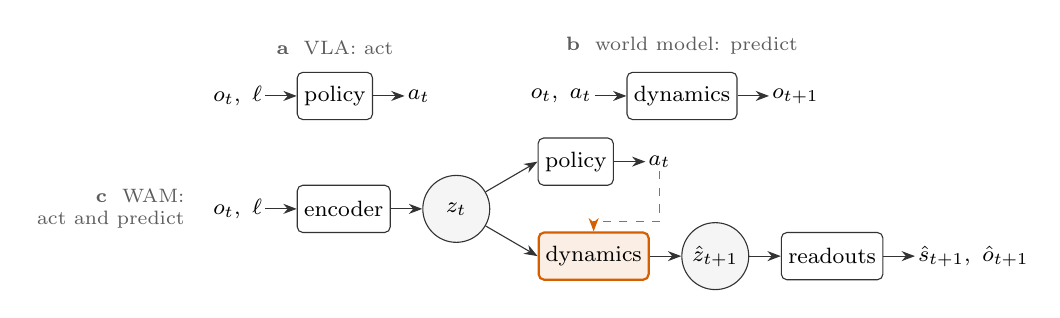
\begin{tikzpicture}[node distance=2.5mm and 4mm]
  % (a) VLA
  \node[io] (o1) {$o_t,\ \ell$};
  \node[box, right=of o1] (p1) {policy};
  \node[io, right=of p1] (a1) {$a_t$};
  \draw[flow] (o1) -- (p1); \draw[flow] (p1) -- (a1);
  \node[lbl, above=1mm of p1] {\textbf{a}\ \ VLA: act};
  % (b) world model
  \node[io, right=12mm of a1] (o2) {$o_t,\ a_t$};
  \node[box, right=of o2] (f2) {dynamics};
  \node[io, right=of f2] (s2) {$o_{t+1}$};
  \draw[flow] (o2) -- (f2); \draw[flow] (f2) -- (s2);
  \node[lbl, above=1mm of f2] {\textbf{b}\ \ world model: predict};
  % (c) WAM
  \node[io, below=11mm of o1] (o3) {$o_t,\ \ell$};
  \node[box, right=of o3] (e3) {encoder};
  \node[lat, right=of e3] (z3) {$z_t$};
  \node[box, right=6mm of z3, yshift=6mm] (p3) {policy};
  \node[io, right=of p3] (a3) {$a_t$};
  \node[ours, right=6mm of z3, yshift=-6mm] (f3) {dynamics};
  \node[lat, right=of f3] (z31) {$\hat z_{t+1}$};
  \node[box, right=of z31] (r3) {readouts};
  \node[io, right=of r3] (y3) {$\hat s_{t+1},\ \hat o_{t+1}$};
  \draw[flow] (o3) -- (e3); \draw[flow] (e3) -- (z3);
  \draw[flow] (z3) -- (p3.west); \draw[flow] (z3) -- (f3.west);
  \draw[flow] (p3) -- (a3); \draw[flow] (f3) -- (z31); \draw[flow] (z31) -- (r3); \draw[flow] (r3) -- (y3);
  \draw[aflow] (a3.south) |- ($(f3.north)+(0,1.2mm)$) -- (f3.north);
  \node[lbl, left=2mm of o3, anchor=east, align=right] {\textbf{c}\ \ WAM:\\act and predict};
\end{tikzpicture}
\caption{\textbf{Policy prediction, forward prediction, and joint training.} (a) A policy maps observation $o_t$ and instruction $\ell$ to action $a_t$. (b) An action-conditioned forward model predicts a future observation. (c) In pico-WAM, a policy and transition model share latent state $z_t$. The transition model accepts a specified action, and readouts convert its predicted latent into a physical state and image. Repeated transitions generate an open-loop rollout. The reactive policy does not use this rollout to select actions; the Push-T planner does.}
\label{fig:paradigms}
\end{figure}

Several recent WAMs use billion-parameter video backbones \citep{liao2025genie,kim2026cosmospolicy,li2026lingbotva}, making controlled comparisons expensive. Tutorials describe their design choices \citep{zhang2026tutorial}, and minimal video-prediction implementations simplify some components \citep{huang2026nano}. A small model containing both a policy and a predictor allows their interaction to be tested directly.

We present pico-WAM, a model of about a million parameters with image, instruction, and state encoders, an action head, latent dynamics, and state and image decoders: 0.75M in the point-mass study, and \PTfinalParamsWamM M on Push-T, where a larger action head accounts for the difference. We study it in two environments whose simulators can replay any alternative action exactly. A point-mass navigation task has affine dynamics and a fully known state, which makes each effect easy to isolate. Push-T \citep{chi2023diffusion} requires pushing a T-shaped block onto a target through frictionless contact, and we train on its 206 human demonstrations. In both, we ask whether prediction along recorded trajectories generalizes to other actions, whether auxiliary prediction improves the policy, whether the world model is accurate enough to plan with, and which components account for the cost.

The paper compares eight open-source systems, evaluates data coverage and training objectives in both environments, tests planning with the learned dynamics on Push-T, and profiles parameters and runtime. The architecture uses established components; the contribution is an implementation and an empirical study of their behavior at a scale where every prediction can be checked against a simulator.

% =====================================================================
\section{Prediction and control in existing systems}
\label{sec:design}

We compare systems along four dimensions: the prediction target, the relation between actions and predictions, the model architecture, and the use of predicted futures (Figure~\ref{fig:design}). These dimensions describe design choices rather than mutually exclusive model classes. For example, joint training can include an action-conditioned forward model, and a video model can serve both as a predictor and as a source of synthetic data. Table~\ref{tab:wams} includes such related systems alongside joint policy--prediction models.

\begin{figure}[!htbp]
\centering
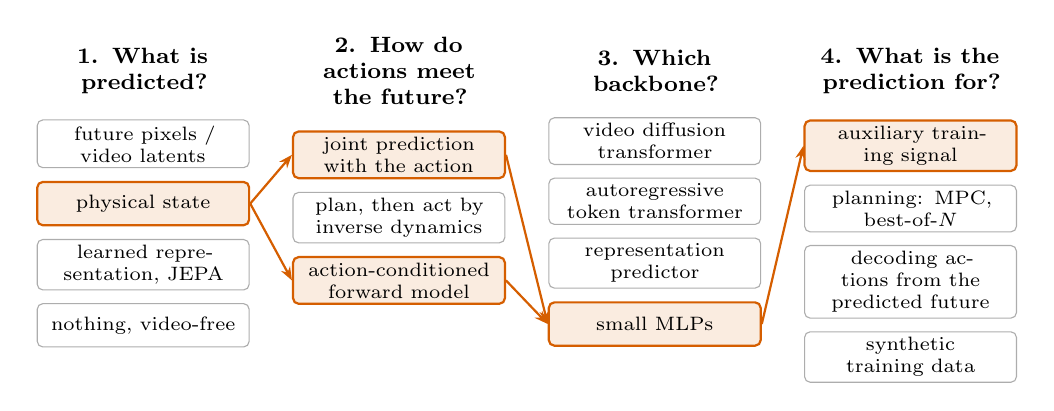
\begin{tikzpicture}[node distance=1.6mm and 3mm]
  \node[head] (h1) {1. What is predicted?};
  \node[head, right=of h1] (h2) {2. How do actions meet the future?};
  \node[head, right=of h2] (h3) {3. Which backbone?};
  \node[head, right=of h3] (h4) {4. What is the prediction for?};
  % column 1
  \node[opt, below=2mm of h1] (c11) {future pixels / video latents};
  \node[pick, below=of c11] (c12) {physical state};
  \node[opt, below=of c12] (c13) {learned representation, JEPA};
  \node[opt, below=of c13] (c14) {nothing, video-free};
  % column 2
  \node[pick, below=2mm of h2] (c21) {joint prediction with the action};
  \node[opt, below=of c21] (c22) {plan, then act by inverse dynamics};
  \node[pick, below=of c22] (c23) {action-conditioned forward model};
  % column 3
  \node[opt, below=2mm of h3] (c31) {video diffusion transformer};
  \node[opt, below=of c31] (c32) {autoregressive token transformer};
  \node[opt, below=of c32] (c33) {representation predictor};
  \node[pick, below=of c33] (c34) {small MLPs};
  % column 4
  \node[pick, below=2mm of h4] (c41) {auxiliary training signal};
  \node[opt, below=of c41] (c42) {planning: MPC, best-of-$N$};
  \node[opt, below=of c42] (c43) {decoding actions from the predicted future};
  \node[opt, below=of c43] (c44) {synthetic training data};
  \draw[wam, thick, -{Stealth[length=1.7mm]}] (c12.east) -- (c21.west);
  \draw[wam, thick, -{Stealth[length=1.7mm]}] (c12.east) -- (c23.west);
  \draw[wam, thick, -{Stealth[length=1.7mm]}] (c21.east) -- (c34.west);
  \draw[wam, thick, -{Stealth[length=1.7mm]}] (c23.east) -- (c34.west);
  \draw[wam, thick, -{Stealth[length=1.7mm]}] (c34.east) -- (c41.west);
\end{tikzpicture}
\caption{\textbf{Design choices in predictive control systems.} The columns distinguish prediction target, action modeling, architecture, and use of predictions. Orange marks pico-WAM's main configuration: state prediction, joint policy--dynamics training, an action-conditioned MLP transition, and auxiliary supervision. Image decoding is optional. Choices can overlap; for example, a jointly trained model can also support forward prediction under supplied actions. Table~\ref{tab:wams} compares the main configurations of eight related systems.}
\label{fig:design}
\end{figure}

\begin{table}[!htbp]
\centering\footnotesize
\begin{tabularx}{\linewidth}{>{\hsize=0.72\hsize}L >{\hsize=0.98\hsize}L >{\hsize=1.12\hsize}L >{\hsize=0.98\hsize}L >{\hsize=1.2\hsize}L}
\toprule
System & Predicts & Backbone & Action decoding & Future used for \\
\midrule
GR-1 \citep{wu2023gr1} & future frames (image patches) & GPT-style causal transformer, video-pretrained on Ego4D clips & linear head on an \texttt{[ACT]} token & training signal \\
UWM \citep{zhu2025uwm} & video and actions & one diffusion transformer, independent timesteps per modality & action diffusion & policy, forward or inverse dynamics, video generation \\
WorldVLA \citep{cen2025worldvla} & next frame (VQ tokens) & autoregressive multimodal LLM (Chameleon init.) & discrete action tokens & training signal \\
Genie Envisioner \citep{liao2025genie} & video chunks & video diffusion transformer (2B) & flow-matching action module on video latents & action decoding; neural simulator \\
Cosmos Policy \citep{kim2026cosmospolicy} & future states and values as latent frames & Cosmos-Predict2 video diffusion (2B) & actions injected as latent frames & best-of-$N$ planning \\
V-JEPA 2-AC \citep{assran2025vjepa2} & future representations & frozen V-JEPA 2 encoder + 300M action-conditioned predictor & none: actions come from the planner & CEM model-predictive control \\
DreamGen \citep{jang2025dreamgen} & robot videos & fine-tuned video generation model & inverse dynamics or latent actions label the videos & synthetic training data \\
LingBot-VA \citep{li2026lingbotva} & video latents, autoregressively & dual-stream diffusion transformer (5.3B), KV cache & inverse dynamics from the predicted future & action decoding; memory \\
\midrule
\textbf{pico-WAM} (ours) & physical state, pixels, latents & 3-layer CNN + GRU + MLPs (0.75--1.3M) & MLP, diffusion or flow head & training signal; analysis \\
\bottomrule
\end{tabularx}
\caption{\textbf{Comparison of eight open-source predictive robot-learning systems and pico-WAM.} Entries describe the main configuration reported in each paper. The table includes joint policy models, forward models used by planners, and video generators used to create training data. Their prediction targets and deployment roles differ, so model size alone is not a comparison of capability.}
\label{tab:wams}
\end{table}

These deployment roles require different evaluations. Auxiliary prediction should be judged by its effect on the deployed policy; planning additionally requires accurate comparisons between candidate actions. Synthetic-data methods must be evaluated through policies trained on their generated data. pico-WAM studies the first setting and tests its forward model separately.

GR-1's future-frame objective \citep{wu2023gr1}, Cosmos Policy's action selection \citep{kim2026cosmospolicy}, and V-JEPA 2-AC's representation-space planning \citep{assran2025vjepa2} motivate our tests of prediction horizon, action coverage, and decoding cost. Planning with learned dynamics has also been studied on Push-T itself. DINO-WM plans with a cross-entropy method in the patch features of a frozen DINOv2 encoder, using a predictor of about 19M parameters trained on 18,500 trajectories \citep{zhou2024dinowm}. PILOT initializes the cross-entropy method from a learned policy and reports gains over executing the same policy on long Push-T tasks \citep{liu2026pilot}. AD-WM finds that factual prediction error does not follow closed-loop planning success \citep{qiu2026adwm}, and SufficientPlan reports competitive control with much smaller search budgets than are usually used \citep{li2026sufficientplan}. We test the same questions with a model trained from scratch whose every component, encoder included, totals about a fourteenth of DINO-WM's predictor alone, and in an environment where the planner's predictions can be compared with the simulator's at every step. Small settings make these choices inexpensive to examine, but cannot establish that the same mechanisms explain results in large robot models.

% =====================================================================
\section{Model and experimental setup}
\label{sec:build}

\begin{figure}[!htbp]
\centering
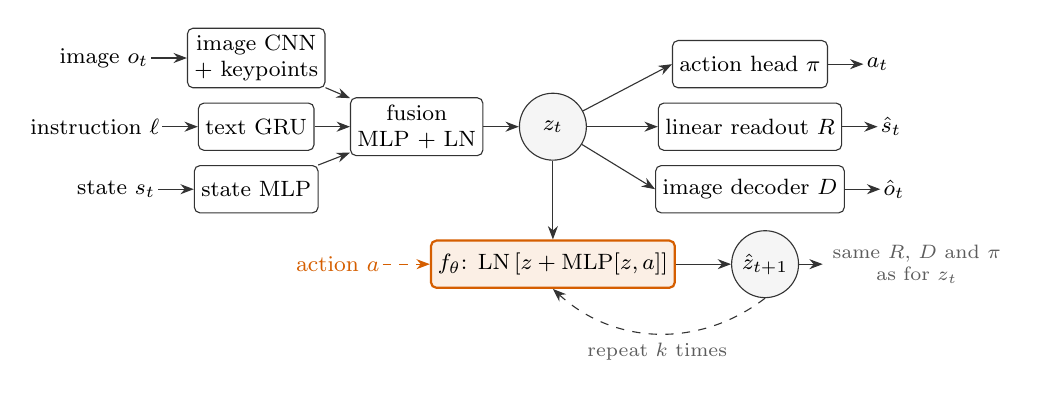
\begin{tikzpicture}[node distance=2.5mm and 4.5mm]
  \node[box] (te) {text GRU};
  \node[box, above=1.8mm of te] (ie) {image CNN\\+ keypoints};
  \node[box, below=1.8mm of te] (se) {state MLP};
  \node[io, left=of ie] (img) {image $o_t$};
  \node[io, left=of te] (txt) {instruction $\ell$};
  \node[io, left=of se] (st) {state $s_t$};
  \node[box, right=of te] (fu) {fusion\\MLP + LN};
  \node[lat, right=of fu] (z) {$z_t$};
  \foreach \u/\v in {img/ie, txt/te, st/se, ie/fu, te/fu, se/fu, fu/z} \draw[flow] (\u) -- (\v);
  \node[box, right=9mm of z] (ro) {linear readout $R$};
  \node[box, above=1.8mm of ro] (pol) {action head $\pi$};
  \node[box, below=1.8mm of ro] (dec) {image decoder $D$};
  \foreach \v in {pol, ro, dec} \draw[flow] (z) -- (\v.west);
  \node[io, right=of pol] (a) {$a_t$};
  \node[io, right=of ro] (sh) {$\hat s_t$};
  \node[io, right=of dec] (ih) {$\hat o_t$};
  \draw[flow] (pol) -- (a); \draw[flow] (ro) -- (sh); \draw[flow] (dec) -- (ih);
  \node[ours, below=10mm of z] (dyn) {$f_\theta$: $\mathrm{LN}\,[z + \mathrm{MLP}[z, a]]$};
  \node[io, left=6mm of dyn, text=wam] (act) {action $a$};
  \node[lat, right=7mm of dyn] (z1) {$\hat z_{t+1}$};
  \draw[flow] (z) -- (dyn); \draw[aflow] (act) -- (dyn); \draw[flow] (dyn) -- (z1);
  \node[lbl, right=3mm of z1] (z1out) {same $R$, $D$ and $\pi$\\as for $z_t$};
  \draw[flow] (z1) -- (z1out);
  \draw[flow, dashed] (z1.south) to[bend left=40] node[lbl, below] {repeat $k$ times} (dyn.south);
\end{tikzpicture}
\caption{\textbf{pico-WAM architecture.} Image, instruction, and state encoders produce features that are fused into $z_t$. The action head, linear state readout $R$, and image decoder $D$ use this representation. The residual transition model $f_\theta$ predicts the next latent from $(z_t,a_t)$; the same readouts decode subsequent latents. Layer normalization controls latent scale but does not ensure that predicted and encoded latents have identical distributions. Figure~\ref{fig:efficiency} reports parameter counts.}
\label{fig:arch}
\end{figure}

\paragraph{Architecture.} The observation comprises a $64\times64$ RGB image $o_t$, an instruction $\ell$, and, when available, a low-dimensional state $s_t$: six numbers for the point mass and eight for Push-T. A three-layer CNN, a text GRU, and a state MLP encode these inputs. The image encoder combines 16 spatial-softmax keypoints with pooled image features. A fusion MLP followed by layer normalization produces $z_t\in\mathbb R^{128}$ (Figure~\ref{fig:arch}).

The policy maps $z_t$ to a two-dimensional action. The implementation supports MLP, diffusion, and flow heads, optionally predicting a chunk of the next $K$ actions. The point-mass experiments use an MLP head with one hidden layer of 128 units and $K=1$. On Push-T, the final configuration uses three hidden layers of 512 units and predicts $K=8$ actions, executing the first four before predicting again, as in Diffusion Policy \citep{chi2023diffusion}. The transition model is a residual MLP, $f_\theta(z,a)=\operatorname{LN}(z+\operatorname{MLP}[z,a])$. Starting from $\hat z_t=z_t$, it predicts successive latents through $\hat z_{t+k+1}=f_\theta(\hat z_{t+k},a_{t+k})$. A linear readout $R$ predicts the normalized physical state, and a decoder $D$ predicts an image residual relative to the training-set mean image. Both readouts apply to encoded and predicted latents. Because $R$ is trained with state labels, its accuracy measures supervised state reconstruction, not independently discovered physical structure.

\paragraph{Training objective.} Each sample is a window of $H$ transitions from one episode. The model encodes the initial observation and predicts the next $H$ latents using the recorded actions (Figure~\ref{fig:train}). Training minimizes
\begin{equation}
\mathcal L=\mathcal L_{\mathrm{act}}+w_s\mathcal L_{\mathrm{state}}
+w_i\mathcal L_{\mathrm{image}}+w_z\mathcal L_{\mathrm{latent}}.
\label{eq:loss}
\end{equation}
The state loss adds current-state reconstruction MSE to mean future-state MSE across the $H$ predictions; the image loss has the same form. The latent loss averages MSE between predicted latents and stop-gradient encodings of the corresponding future observations. All MSE terms average over output coordinates. State targets use training-set means and standard deviations. The default weights are $w_s=0.5$ and $w_i=w_z=1$, with $H=5$.

The action loss is evaluated only on expert-labeled transitions. Removing the transition model, the readouts and their losses leaves mini-VLA \citep{pandya2025minivla}, the small vision-language-action model whose encoders pico-WAM extends, and we use it as the behavioral-cloning comparator. It shares pico-WAM's image encoder and action head, so the two models differ only in the world model and its losses, and it is trained from scratch on the same demonstrations. At deployment, both policies encode the current observation and emit an action; neither uses imagined states to select that action.

\begin{figure}[!htbp]
\centering
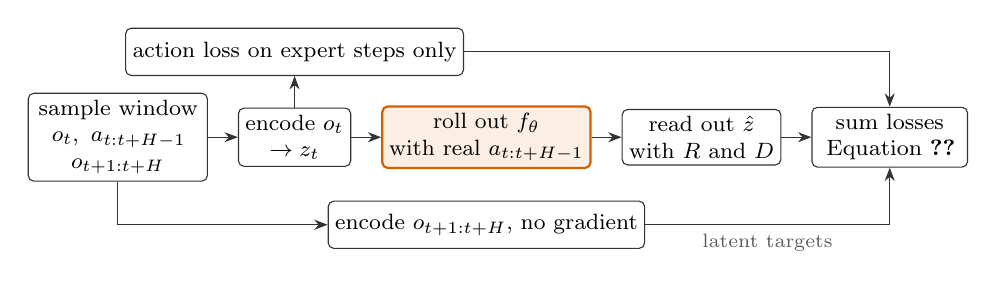
\begin{tikzpicture}[node distance=2.5mm and 3.8mm]
  \node[box, text width=2.1cm] (win) {sample window\\$o_t,\ a_{t:t+H-1}$\\$o_{t+1:t+H}$};
  \node[box, right=of win] (enc) {encode $o_t$\\$\rightarrow z_t$};
  \node[ours, right=of enc] (roll) {roll out $f_\theta$\\with real $a_{t:t+H-1}$};
  \node[box, right=of roll] (read) {read out $\hat z$\\with $R$ and $D$};
  \node[box, right=of read, text width=1.8cm] (loss) {sum losses\\Equation~\ref{eq:loss}};
  \draw[flow] (win) -- (enc); \draw[flow] (enc) -- (roll); \draw[flow] (roll) -- (read); \draw[flow] (read) -- (loss);
  \node[box, below=4mm of roll] (tgt) {encode $o_{t+1:t+H}$, no gradient};
  \draw[flow] (win.south) |- (tgt.west);
  \draw[flow] (tgt.east) -| node[lbl, pos=0.25, below] {latent targets} (loss.south);
  \node[box, above=4mm of enc] (pol) {action loss on expert steps only};
  \draw[flow] (enc.north) -- (pol.south);
  \draw[flow] (pol.east) -| (loss.north);
\end{tikzpicture}
\caption{\textbf{Training on a window of $H$ transitions.} The initial observation is encoded with gradients, and the transition model is rolled forward using recorded actions. State and image readouts are trained against current and future targets. Future observations are encoded to form stop-gradient targets for latent consistency; they are not inputs to the rollout. The action loss uses only expert-labeled steps, whereas prediction losses use all sampled transitions.}
\label{fig:train}
\end{figure}

\paragraph{Point-mass navigation.} The agent moves toward one of two colored goals selected by the instruction (Figure~\ref{fig:toy}). Position $p_t$ lies in the unit square, action $a_t\in[-1,1]^2$ applies a force, and physical velocity follows
\[
v_{t+1}=0.8v_t+0.01a_t,\qquad
p_{t+1}=\operatorname{clip}(p_t+v_{t+1},0,1).
\]
The observed state is $(p_t,v_t/0.05,g)$, where $g$ is the selected goal position. Success requires distance to $g$ below 0.05 and normalized speed below 0.2. A proportional--derivative controller supplies expert actions. When no random burst is active, the collector starts one with probability 0.3; its duration is sampled uniformly from one to three steps. Each burst action is sampled uniformly from $[-1,1]^2$. Thus 0.3 is the burst-start probability, not the fraction of random transitions.

In the state-input condition, the selected goal coordinates already identify the target, so the policy need not use language to select it. In the pixel-input condition, the state-encoder output is set to zero, but the WAM still receives state-prediction targets during training. Velocity is not rendered: one image can correspond to different velocities. We therefore distinguish pixel inputs from training without state supervision.

\begin{figure}[!htbp]
\centering
\includegraphics{\figpath/fig-toy-world.pdf}
\caption{\textbf{Navigation environment and data collection.} (a) Actual frames from an expert episode. The red agent must reach the instructed goal and slow down; the other colored square is a distractor. Images show positions but not velocity. (b) Actions from a collection episode, with random-action bursts shaded. When no burst is active, one starts with probability 0.3 and lasts one to three steps. These transitions contribute to prediction losses but are excluded from action regression.}
\label{fig:toy}
\end{figure}

\paragraph{Push-T.} The agent is a disk of radius 15\,px that tracks a target point with a proportional--derivative controller in a $512\times512$ workspace. It pushes a T-shaped block, a $120\times30$ bar over a $30\times90$ stem, onto a fixed target pose through frictionless contact (Figure~\ref{fig:pusht}). Physics runs at 100\,Hz and control at 10\,Hz with the original constants \citep{chi2023diffusion}. We make two changes. An action $a_t\in[-1,1]^2$ moves the controller's target up to 100\,px from the agent instead of placing it at an absolute position, so a random action is a local nudge and a constant action pushes in one direction. The block's velocity is also reset at every control step; under the original zero damping it carries over for only one 10\,ms substep. With this change, the observed state determines the next one: re-simulating from a recorded state reproduces the next state exactly. The eight-dimensional state holds the agent's position and velocity and the block's position and orientation, $\cos\theta$ and $\sin\theta$, in the unit square. Images are drawn like the dataset's frames, on a $512\times512$ canvas resized to $96\times96$ and then to $64\times64$. Success requires the block to cover more than 95\% of the target; we also report the best coverage reached in an episode, the benchmark's usual score.

The training data are the 206 human demonstrations of LeRobot's Push-T dataset, 25,650 frames at 10\,Hz \citep{lerobot}. The dataset records the agent's position and an absolute target position, but not the block. We read the block's pose from the T's corners in the dataset's keypoint version, recover the agent's velocity by replaying the controller from rest, which reproduces every recorded position to within $10^{-4}$\,px, and convert each target into a relative action; \PTdataClipped{} targets lie more than 100\,px away on an axis and are clipped. Dropping each episode's last frame leaves 25,444 transitions. From a recorded state, our simulator predicts the next recorded block position to within \PTdataBlockErrPninetynine\,px in 99\% of steps, while a moving block travels a median \PTdataBlockMove\,px per step. The demonstrations never reach the success threshold: their best coverage averages \PTdataDemoCoverage\%. For data-coverage experiments we also collect 200 episodes per run with a scripted expert that chooses each push by simulating about a hundred candidates and walks around the block to make it. Random-action bursts start with probability $p$, as in the point-mass task, and draw each action from the whole action range. The expert succeeds in \PTexpertZeroSuccess\% of 30 test starts without bursts, but in only \PTexpertTenthSuccess\% at $p=0.1$: a random action can undo the final placement.

\begin{figure}[!htbp]
\centering
\includegraphics{\figpath/fig-pusht-task.pdf}
\caption{\textbf{Push-T.} (a) Frames of an unseen human demonstration from LeRobot's dataset, as the model sees them. The blue agent must push the grey T onto the green target. (b) Actions of a scripted-expert episode with random-action bursts shaded, at burst-start probability 0.3. An action moves the controller's target by up to 100\,px from the agent on each axis.}
\label{fig:pusht}
\end{figure}

\paragraph{Planning with the world model.} On Push-T we also let the WAM act by planning with its own dynamics. At each step the planner encodes $o_t$, imagines the policy's own next 12 actions, and samples 256 candidate sequences around them with Gaussian noise of standard deviation 0.1, always including the policy's plan itself. Each candidate is rolled out with $f_\theta$, and $R$ reads the predicted block pose at every step. A candidate's cost is the mean distance in pixels between the T's corners and the target's corners, averaged over the 12 steps with weights rising from 0.5 to 1.5, plus 0.05 times the distance between the agent and the block. The first action of the cheapest candidate is executed, and the next step's search starts again from the policy. Our first planner instead started each search from the previous step's plan, shifted by one step, and kept that plan unless a candidate scored better; we call it the warm-start planner and compare the two below. The planner never calls the simulator. Its settings were fixed on 20 development starts, which are never used for testing. Figure~\ref{fig:pusht-planner} shows one planning step of the final model.

Every 10 steps of a planning episode, we also check the chosen plan: from the same state, the simulator executes the whole 12-step plan open loop. Distances between block poses are mean distances between the T's eight corners, in pixels, as in the planner's cost. The check reports the distance between the imagined and the simulated final pose, which we call plan error, and how much closer to the target the model expected the plan to bring the block, against how much closer it really came.

\begin{figure}[!htbp]
\centering
\includegraphics{\figpath/fig-pusht-planner.pdf}
\caption{\textbf{One planning step.} (a) From the current state, the world model imagines 256 action sequences of 12 steps around the policy's own plan; grey lines are the agent paths it imagines for every fourth candidate. The chosen plan has the lowest imagined cost. Its imagined final T pose, dashed, is close to the pose the simulator produces for the same actions, solid. Only the first action is executed before the search starts again. (b) Imagined costs of all 256 candidates: the mean distance between the T's corners and the target's over the 12 steps, plus a small pull of the agent toward the T.}
\label{fig:pusht-planner}
\end{figure}

\paragraph{Evaluation protocol.} Each configuration uses three independent split and initialization seeds and a 90/10 episode split, and trains for 15 epochs unless stated otherwise; the final Push-T configuration trains for 100. In the point-mass task each seed also collects its own 400 episodes; on Push-T the human demonstrations are the same in every run, and scripted data are collected per seed. Closed-loop evaluation uses 100 unseen starts per run, of 80 steps for the point mass and 300 for Push-T. Prediction is evaluated on unseen episodes by encoding each valid starting observation once and rolling forward without observing later frames. Factual evaluation uses recorded actions. Counterfactual evaluation samples eight random action sequences at starts spaced five steps apart and compares each prediction with the simulator. Random actions span the full action range in the point-mass task and up to 40\,px on each axis on Push-T, about twice a typical human action.

State error is mean squared error after dividing each coordinate's residual by its training-set standard deviation, written nMSE. Factual error averages all state coordinates. Point-mass counterfactual error averages position and velocity, the coordinates that actions move; on Push-T it averages all eight, and we also report the four block coordinates separately. Image error is pixel MSE on RGB values scaled to $[0,1]$. Factual persistence repeats the initial state or image. The counterfactual reference instead runs the true simulator with zero actions from the same initial state.

The main studies report population standard deviations over three runs; the five-run supervision pilots report sample standard deviations. These are measures of run-to-run variation, not confidence intervals. Overlapping prediction windows are correlated. Exploration conditions also change state distributions and normalization statistics, so their errors describe the resulting datasets rather than an isolated effect of action diversity.

% =====================================================================
\section{Point-mass results}
\label{sec:lessons}

We first evaluate the forward model, then examine whether auxiliary prediction improves the policy. Table~\ref{tab:lessons} summarizes the main comparisons. It also records decoder and diffusion-schedule changes made during development; those observations are distinguished from the repeated experimental comparisons.

\begin{table}[!htbp]
\centering\footnotesize
\begin{tabularx}{\linewidth}{>{\hsize=0.7\hsize}L >{\hsize=1.0\hsize}L >{\hsize=1.5\hsize}L >{\hsize=0.8\hsize}L}
\toprule
Component & Comparison & Observation & Interpretation \\
\midrule
Training data & expert only vs.\ burst-start probability 0.3 & counterfactual error at $k{=}10$ falls from $0.112$ to $0.0072$, even though factual error is lower with expert-only data (Fig.~\ref{fig:coverage}) & lower counterfactual error \\
Imagination horizon $H$ & 1, 5, 10 steps & 10-step counterfactual error $0.0139$, $0.0072$, $0.0057$; one-step error $0.0019$, $0.0019$, $0.0030$ & short-/long-horizon trade-off \\
Latent consistency & on vs.\ off & 15-step error $0.0071\pm0.0004$ vs.\ $0.0096\pm0.0024$; one-step error slightly better without it & lower long-horizon error and spread \\
Image loss & on vs.\ off (state input) & 15-step state error $0.0071$ vs.\ $0.0074$ & similar observed means \\
Decoder output & sigmoid vs.\ residual on the mean image & sigmoid training stalled; the residual decoder learns, but remains worse than frame copying (Fig.~\ref{fig:imagine}c) & limited image fidelity \\
Visual representation & keypoints with vs.\ without state input & with state input the keypoints barely move; without it they track the agent, $R^2 \ge 0.998$ & stronger localization without state input \\
Diffusion head & linear schedule ($\bar\alpha_T \approx 0.92$) vs.\ cosine ($\bar\alpha_T \approx 10^{-5}$) & the linear schedule never reaches noise, yet sampling starts from noise; fixed with a cosine schedule and the DDPM posterior & noise-schedule correction \\
Auxiliary supervision & BC, + current state, + future state (pixel input) & success $17.0\%$, $28.4\%$, $33.6\%$; current-state supervision gives the larger increment (Fig.~\ref{fig:policy}c) & future prediction adds 5.2 points \\
Few demonstrations & 25 to 400 episodes & WAM trails mini-VLA at 25 episodes ($87\%$ vs.\ $99.7\%$); matched updates close most of the gap & sensitive to update budget \\
\bottomrule
\end{tabularx}
\caption{\textbf{Experimental comparisons and implementation observations.} State errors are normalized MSE, and policy success is measured on 100 unseen episodes per run. Main comparisons use three runs; the supervision pilot uses five. Decoder and diffusion-schedule rows describe development observations, not repeated ablations. Factual error averages six state coordinates; counterfactual error averages position and velocity only. Similar means do not establish equivalence.}
\label{tab:lessons}
\end{table}

\paragraph{State and image prediction.} At horizon 15, factual state NMSE is $0.0071\pm0.0004$, compared with $0.5824$ for persistence. At horizon 10, counterfactual error is $0.0072$, compared with $0.388$ for the zero-action simulator reference (Figure~\ref{fig:imagine}). The model therefore predicts motion substantially better than these references. The comparison does not establish an advantage over a fitted state-space model.

Image prediction is less successful. Pixel MSE exceeds frame copying at every evaluated horizon, despite accurate state readouts. In an unseen example episode, the decoder retains the agent and selected goal but fails to reconstruct the distractor. This example illustrates a reconstruction failure; it does not establish why the distractor is lost. The large static background also makes copying a strong pixel baseline.

\begin{figure}[!htbp]
\centering
\includegraphics{\figpath/fig-imagination-quality.pdf}
\caption{\textbf{Prediction error versus rollout horizon.} (a) Factual normalized state MSE compared with persistence. (b) Counterfactual normalized MSE under random actions, compared with a true-simulator rollout that applies zero actions. (c) Pixel MSE compared with repeating the initial frame. Lines show means and bands population standard deviations across three runs, each with 40 unseen episodes. State prediction improves on these references; image prediction does not.}
\label{fig:imagine}
\end{figure}

\paragraph{Prediction under alternative actions.} Expert-only training gives lower long-horizon factual error but a counterfactual error of $0.112$ at horizon 10, versus $0.0072$ with burst-start probability 0.3 (Figure~\ref{fig:coverage}). Accurate prediction along expert trajectories therefore does not imply equally accurate prediction under other actions. A network may exploit correlations between states and expert actions, as discussed in work on causal confusion \citep{dehaan2019causal}; this experiment does not directly measure whether the network ignores its action input.

A separate five-run diagnostic fits an affine state-and-action predictor, with the known position-clipping rule, to deterministic expert trajectories. Its ten-step counterfactual position MSE is approximately $4.3\times10^{-16}$. Expert data therefore identifies the transition within this restricted model class. The neural result reflects the interaction between data and model fitting, rather than an unavoidable lack of information in the demonstrations. These raw position errors are not directly comparable with neural NMSE.

\begin{figure}[!htbp]
\centering
\includegraphics{\figpath/fig-exploration.pdf}
\caption{\textbf{Effect of the data-collection policy.} (a) Ten-step factual and counterfactual errors at different burst-start probabilities. Expert-only data gives lower factual error but higher counterfactual error. Grey marks the zero-action simulator reference. (b) Closed-loop success remains high across these conditions; only expert-labeled steps contribute to imitation. Dots denote runs and bars population standard deviations over three runs. The horizontal setting controls burst initiation, not the measured fraction of random steps; trajectory distributions also change.}
\label{fig:coverage}
\end{figure}

\paragraph{Sustained-action prediction.} We also evaluate 15 consecutive steps of constant force, longer than the one-to-three-step random bursts in training. Figure~\ref{fig:whatif} compares predicted and simulated trajectories from one initial state. Several predictions underestimate displacement. Across unseen episode starts, mean endpoint distance is $0.103\pm0.010$ in unit-square coordinates, compared with $0.457$ when every action is assigned the zero-force endpoint. The model captures much of the action-dependent displacement but retains appreciable long-horizon error.

\begin{figure}[!htbp]
\centering
\includegraphics{\figpath/fig-what-if.pdf}
\caption{\textbf{Predictions under sustained force.} (a) Predicted (dashed) and simulated (solid) trajectories for 15 steps of constant force in eight directions, plus a zero-force condition. (b) Predicted final frames, arranged by force direction. (c) Endpoint distances averaged over the initial states of 40 unseen episodes per run; whiskers show population standard deviations across three runs. Grey bars assign the zero-force endpoint to every action sequence.}
\label{fig:whatif}
\end{figure}

\paragraph{Visual representations.} With state inputs, the 16 spatial-softmax keypoints vary little and remain near the image center. Removing state inputs produces keypoints that track the agent and goals; the best-keypoint tracking score is $R^2\ge0.998$ in each run. This is consistent with greater reliance on visual localization when positions are not supplied directly. It is not a controlled comparison between spatial-softmax and global-pooling encoders.

\paragraph{Policy performance.} With state inputs and 400 episodes, both WAM and mini-VLA achieve 100\% success. With 25 episodes and 15 epochs, WAM achieves 87.0\%, compared with 99.7\% for mini-VLA. Extending training to 225 epochs narrows this difference to 96.3\% versus 98.7\% (Figure~\ref{fig:policy}a). Update budget is therefore an important factor in the low-data comparison.

With pixel inputs, success is $80.3\pm12.0\%$ for WAM and $36.0\pm19.8\%$ for mini-VLA (Figure~\ref{fig:policy}b). WAM performs better in all three runs, but it also receives state targets that mini-VLA does not. In addition, the original WAM uses five-step training windows, while mini-VLA uses one-step windows. These windows exclude different episode-end samples.

To separate current-state supervision from future prediction, a five-run Explorer pilot uses 200 episodes per run, 15 epochs, and matched five-step starts, initialization, batches, and update counts. Success is 17.0\% for cloning alone, 28.4\% with current-state supervision, and 33.6\% with current and future-state supervision (Figure~\ref{fig:policy}c). The increments are 11.4 and 5.2 percentage points; the latter ranges from $-2$ to $+9$ points across runs. The pilot excludes image and latent-consistency losses. Its lower data budget and different objective prevent attributing the original 44.3-point gap to the same proportions.

\begin{figure}[!htbp]
\centering
\includegraphics{\figpath/fig-policy.pdf}
\caption{\textbf{Policy success under different data and supervision conditions.} (a) Success versus collected episode count after 15 epochs. Open markers use 225 epochs on 25 episodes to approximately match the standard update budget. (b) State-input and pixel-input policies trained on 400 episodes, with dots for individual runs. (c) Matched pixel-input pilot on 200 episodes per run: cloning, current-state supervision, and current plus five-step future-state supervision. Grey lines connect five runs; orange shows mean and sample SD. Panels (a,b) use three runs and the full WAM objective; panel (c) excludes image and latent-consistency losses.}
\label{fig:policy}
\end{figure}

% =====================================================================
\section{Push-T results}
\label{sec:pusht}

We first evaluate the world model against simple references, including a linear model fitted to the same data, then compare reactive policies with planning.

\paragraph{Prediction along human actions.} On unseen demonstrations, pico-WAM predicts the state 15 steps ahead with nMSE \PTbaseStateFifteen, against \PTbaseCopyFifteen{} for persistence (Figure~\ref{fig:pusht-prediction}a). A linear model of the state change, fitted by least squares on the same training transitions from the state and action, is more accurate one step ahead, \PTlinFactOne{} against \PTbaseStateOne, because the agent follows a linear controller. It is less accurate after 15 steps, \PTlinFactFifteen, once contact has moved the block. Decoded images are worse than copying the current frame one step ahead, \PTbaseImgOne{} against \PTbaseImgCopyOne, and better after 15 steps, \PTbaseImgFifteen{} against \PTbaseImgCopyFifteen, once the scene has changed.

\paragraph{Prediction under other actions.} Under random actions, the counterfactual error after 10 steps is \PTbaseCf, against \PTbaseNoop{} for the zero-action reference and \PTlinCf{} for the linear model (Figure~\ref{fig:pusht-prediction}b). The average hides a difference between the two objects. On the block's four coordinates alone, the WAM's error is \PTbaseCfBlock, higher than the \PTbaseNoopBlock{} obtained by assuming the block stays where the zero-action simulator leaves it; the linear model reaches \PTlinCfBlock. Along recorded human actions the block error after 10 steps is \PTbaseFactBlock. The world model has learned how the block moves under the pushes people made, more than how it responds to others. Sustained pushes show the same pattern. After 15 steps of constant pushing in each of eight directions, the predicted agent endpoint is off by \PTwhatifAgent{} of the workspace width, against \PTwhatifAgentIgnore{} if the push is ignored, while the predicted block endpoint is off by \PTwhatifBlock, against \PTwhatifBlockIgnore{} if the push is ignored.

\begin{figure}[!htbp]
\centering
\includegraphics{\figpath/fig-pusht-prediction.pdf}
\caption{\textbf{Push-T prediction error versus rollout horizon.} (a) Factual nMSE along unseen human demonstrations, against persistence and a linear model of state and action fitted to the same data. (b) Counterfactual nMSE under random actions within 40\,px, against the zero-action simulator and the linear model. (c) Pixel MSE against repeating the initial frame. Lines show means and bands population standard deviations across three runs, each with 21 unseen episodes.}
\label{fig:pusht-prediction}
\end{figure}

\paragraph{Policies and planning.} Acting reactively, the WAM reaches a best coverage of \PTbaseWam\% $\pm$ \PTbaseWamSd, below mini-VLA's \PTbaseVla\% $\pm$ \PTbaseVlaSd. Planning with the same world model raises it to \PTbasePlan\% $\pm$ \PTbasePlanSd, above mini-VLA in each of the three runs. No policy succeeds, and no demonstration does either: the demonstrations' best coverage averages \PTdataDemoCoverage\%.

\paragraph{Search budget.} Figure~\ref{fig:pusht-planning} gives the planner more search on the same trained models, all with the warm-start planner of the study base: noise 0.3 instead of 0.1, three cross-entropy rounds with noise 0.3, or three rounds that start from standing still instead of the policy's plan. Coverage falls each time, from \PTbudgetPlan\% to \PTbudgetPlanWide\%, \PTbudgetPlanCem\% and \PTbudgetPlanNoprior\%. The plan checks show why. The improvement the model expects from its chosen plan grows with the search, from \PTbudgetPlanExpected\,px to \PTbudgetPlanCemExpected\,px with three rounds, while the simulated improvement of the same plans stays near zero: \PTbudgetPlanReal, \PTbudgetPlanWideReal, \PTbudgetPlanCemReal{} and \PTbudgetPlanNopriorReal\,px. Plan error grows from \PTbudgetPlanPlanErr{} to \PTbudgetPlanNopriorPlanErr\,px. A stronger search finds the actions whose outcome the model gets most wrong. This agrees with PILOT's use of a policy prior \citep{liu2026pilot} and with SufficientPlan's finding that small budgets suffice \citep{li2026sufficientplan}; the simulator lets us measure the cause directly.

\begin{figure}[!htbp]
\centering
\includegraphics{\figpath/fig-pusht-planning.pdf}
\caption{\textbf{More search exploits the world model's errors.} (a) Best coverage of the reactive WAM and of four planners using the same models: the default, noise 0.3, three cross-entropy rounds with noise 0.3, and three rounds that start from standing still instead of the policy's plan. The blue band is mini-VLA, mean $\pm$ SD. (b) Every 10 steps, the chosen 12-step plan is executed open loop in the simulator from the same state: how much closer to the target the model expected the block to come, and how much closer it came. Dots are runs, bars population standard deviations over three runs.}
\label{fig:pusht-planning}
\end{figure}

\paragraph{Which data teaches the block's response.} The zero-action reference depends on the test episodes, so we compare datasets by the ratio of the WAM's block error under random actions to that reference on the same starts; below one, the model beats assuming that the block stays put (Figure~\ref{fig:pusht-data}). Trained on human demonstrations, the ratio is \PTbaseCfBlockRatio. Trained on the scripted expert it is \PTexpzCfBlockRatio{} without random bursts, and \PTexponeCfBlockRatio{} and \PTexpthreeCfBlockRatio{} with bursts at $p=0.1$ and $0.3$; human demonstrations plus scripted episodes with bursts at $p=0.3$ give \PTmixedCfBlockRatio. The scripted expert pushes from many contact points because it searches over candidate pushes, and bursts add further actions. The policies do not improve with it. On scripted data mini-VLA reaches \PTexpzVla\% to \PTexponeVla\%, against \PTbaseVla\% on human demonstrations, and planning reaches \PTexponePlan\% to \PTexpthreePlan\%, against \PTbasePlan\%. We did not test why the scripted expert is harder to imitate; one candidate is that its choices depend on a lookahead the policy cannot observe. Planning needs both a world model that knows the block's response and a policy whose plans are worth searching around, which led us to branch the human demonstrations instead (below).

\begin{figure}[!htbp]
\centering
\includegraphics{\figpath/fig-pusht-data.pdf}
\caption{\textbf{Training data and the block's response.} (a) Block nMSE after 10 steps, under random actions and along recorded actions, with the zero-action simulator on the same starts in grey, for each training dataset. Each dataset is tested on its own unseen episodes. (b) Best coverage of mini-VLA, the reactive WAM and the planning WAM. Scripted data comes from the expert with random bursts starting with probability $p$. Dots are runs, bars population standard deviations over three runs.}
\label{fig:pusht-data}
\end{figure}

\paragraph{Objective and model variants.} The upper group of Figure~\ref{fig:pusht-ablations} varies one setting of the study base. Planning depends on latent consistency: without it, coverage falls to \PTnolatPlan\%, although counterfactual error falls slightly. The image loss is not needed for planning, \PTnoimgPlan\% without it. A one-step training horizon lowers planning to \PThonePlan\%, and ten steps give \PThtenPlan\%. Fewer demonstrations lower every policy: with 100 and 50 of the 206, planning reaches \PTdhundredPlan\% and \PTdfiftyPlan\%. From pixels alone, without state input, coverage drops to about 10\% for every policy, and the world model's state error after 15 steps rises to \PTpixStateFifteen. A diffusion head lowers every policy at this training length, to \PTdiffVla\% for mini-VLA. Doubling the latent width to 256 does not help: planning reaches \PTwidePlan\%, and the block's counterfactual error rises to \PTwideCfBlockRatio{} times the reference.

Predicting chunks of eight actions and executing four, as in Diffusion Policy, raises the reactive WAM to \PTchunkWam\% and mini-VLA to \PTchunkVla\%, with the first successes of the study: \PTchunkWamSucc{} and \PTchunkVlaSucc{} in 300 episodes. Planning with the chunked model reaches \PTchunkPlan\%. The lower group varies this chunked model. Predicting 16 actions and executing eight gives \PTchunkSixteenVla\% for mini-VLA, and averaging overlapping chunks gives \PTchunkEnsembleVla\%; neither improves on $K=8$. Halving the latent width to 64 lowers planning to \PTchunkNarrowPlan\%. Replacing the keypoint encoder with a plain CNN and global average pooling gives \PTchunkCnnVla\% for mini-VLA and \PTchunkCnnPlan\% for planning, within the spread of the runs. Without the image decoder, planning reaches \PTchunkNodecPlan\%, against \PTchunkPlan\% with it, at about a tenth of the training cost (Section~\ref{sec:efficiency}). At 15 epochs, neither a narrower nor a wider latent improves on 128.

\begin{figure}[!htbp]
\centering
\includegraphics{\figpath/fig-pusht-ablations.pdf}
\caption{\textbf{Push-T variants.} Upper group: each row changes one setting of the study base, grey, which predicts one action per step. Lower group: each row changes one setting of the model with action chunks, grey. (a) State nMSE after 15 steps along recorded actions. (b) Counterfactual nMSE of the block after 10 random-action steps; dotted lines mark each group's reference row. (c) Best coverage of the target for mini-VLA, the reactive WAM and the planning WAM. Dots are runs, bars population standard deviations over three runs, 100 unseen starts per run.}
\label{fig:pusht-ablations}
\end{figure}

\paragraph{Training longer, and why planning got worse.} Training the chunked models for 100 epochs instead of 15 raises mini-VLA to \PTchunkEpochsVla\% $\pm$ \PTchunkEpochsVlaSd{} with \PTchunkEpochsVlaSucc{} successes in 300 episodes, and the reactive WAM to \PTchunkEpochsWam\% with \PTchunkEpochsWamSucc{} (Figure~\ref{fig:pusht-recipe}). The world model also improves: its state error after 15 steps falls from \PTchunkStateFifteen{} to \PTchunkEpochsStateFifteen. Planning, however, falls from \PTchunkPlan\% to \PTchunkEpochsPlan\%, and 100 epochs without chunks show the same drop, \PTepochsPlan\%. Both runs used the warm-start planner. On development starts, which are never used for testing, its chosen plans with the 100-epoch model expected to bring the T 74\,px closer to the target in 12 steps while the simulator moved it 7\,px further away. Because the warm-start planner keeps the previous plan unless a candidate scores better, an episode accumulates hundreds of rounds of search: in effect, the stronger search of Figure~\ref{fig:pusht-planning}. Restarting each search from the policy's plan prevents this accumulation. On the same 15-epoch chunked models, the restarting planner reaches \PTchunkRestartPlan\% with \PTchunkRestartPlanSucc{} successes and a plan error of \PTchunkRestartPlanPlanErr\,px, against \PTchunkRestartPlanWarm\% with \PTchunkRestartPlanWarmSucc{} successes and \PTchunkRestartPlanWarmPlanErr\,px for the warm start.

\begin{figure}[!htbp]
\centering
\includegraphics{\figpath/fig-pusht-recipe.pdf}
\caption{\textbf{Changes that make Push-T succeed.} Below the study base, each row adds the changes it names to the model with action chunks, which predicts eight actions and executes four; the seventh row trains the row above it for 100 epochs instead of 15, and the last row also gives both policies an action head with three hidden layers of 512. Planning uses the warm-start planner in the first four rows and the restarting planner in the others. Branched data reaches only the world model, so mini-VLA's differences between those rows are run-to-run variation. (a) Best coverage of the target. (b) Success rate, coverage above 95\%. (c) Block counterfactual nMSE after 10 random-action steps; the dashed line is the zero-action simulator, which assumes the block stays put. Dots are runs, bars population standard deviations over three runs, 100 unseen starts per run.}
\label{fig:pusht-recipe}
\end{figure}

\paragraph{Branching the demonstrations.} The data comparison suggests that the world model needs to see the block respond to pushes people did not make, from states people did visit. We therefore branch the human demonstrations with the simulator. From every fourth state of each training demonstration, we replay the next eight human actions with Gaussian noise of standard deviation 0.3 added and record the outcome. This adds 6,013 branches, or 48,104 transitions, in 34\% of which the block moves (Figure~\ref{fig:pusht-branches}). Branches are marked as non-expert, so only the world model learns from them, and each stays on its source demonstration's side of the train/test split. Mini-VLA does not train on them: their actions are perturbed demonstrations, and imitating them would teach the noise. The simulator is used only to build this data before training, never during planning. With branches, the block's counterfactual error falls from \PTchunkCfBlockRatio{} to \PTchunkBranchCfBlockRatio{} times the zero-action reference, and planning with the warm-start planner reaches \PTchunkBranchPlan\% with \PTchunkBranchPlanSucc{} successes. With branches and the restarting planner together, planning reaches \PTbranchRestartPlan\% $\pm$ \PTbranchRestartPlanSd{} with \PTbranchRestartPlanSucc{} successes, against \PTbranchRestartVla\% and \PTbranchRestartVlaSucc{} for mini-VLA trained in the same runs, and plan error falls to \PTbranchRestartPlanPlanErr\,px.

\begin{figure}[!htbp]
\centering
\includegraphics{\figpath/fig-pusht-branches.pdf}
\caption{\textbf{Branching a human demonstration.} (a) A 32-step stretch of one demonstration: the agent's path and where the person left the T. (b) The same stretch with the branches started along it. Each branch replays the person's next eight actions with Gaussian noise of standard deviation 0.3 and lets the simulator say where the agent and the T end up. Only the world model learns from branches.}
\label{fig:pusht-branches}
\end{figure}

\paragraph{Training for 100 epochs.} Training the model with branches and the restarting planner for 100 epochs, the seventh row of Figure~\ref{fig:pusht-recipe}, lets planning reach \PTbranchRestartEpochsPlan\% $\pm$ \PTbranchRestartEpochsPlanSd{} with \PTbranchRestartEpochsPlanSucc{} successes, against \PTbranchRestartEpochsVla\% and \PTbranchRestartEpochsVlaSucc{} for mini-VLA. On the same models, the warm-start planner reaches only \PTbranchRestartEpochsPlanWarm\% with \PTbranchRestartEpochsPlanWarmSucc{} successes and a plan error of \PTbranchRestartEpochsPlanWarmPlanErr{} against \PTbranchRestartEpochsPlanPlanErr\,px: the drift persists at 100 epochs, and restarting the search removes most of its cost. The reactive WAM stays far behind, at \PTbranchRestartEpochsWam\% with \PTbranchRestartEpochsWamSucc{} successes, \PTbranchRestartEpochsGap{} points below mini-VLA.

\paragraph{The action head was the bottleneck.} Up to this point, both policies used an action head with one hidden layer of 128 units. Figure~\ref{fig:pusht-capacity} varies the head and the latent on top of the 100-epoch model. Three hidden layers of 512 raise every policy: mini-VLA to \PTfinalVla\% with \PTfinalVlaSucc{} successes, the reactive WAM to \PTfinalWam\% with \PTfinalWamSucc, and planning to \PTfinalPlan\% with \PTfinalPlanSucc. The reactive WAM now trails mini-VLA by \PTfinalGap{} points instead of \PTbranchRestartEpochsGap, so the small head, rather than the prediction losses sharing its latent, held the WAM's own policy back. Larger heads do not help further: three layers of 1024 give planning \PTheadWidePlan\% and six layers of 512 give \PTheadDeepPlan\%. A flow-matching head with three layers of 512 lowers both reactive policies, mini-VLA to \PTheadFlowVla\% with \PTheadFlowVlaSucc{} successes, although planning still reaches \PTheadFlowPlan\%. A latent of 256 helps the one-layer head, with planning at \PTlatentWidePlan\% and \PTlatentWidePlanSucc{} successes, but adds nothing to the 3$\times$512 head, \PTheadLatentPlan\% with \PTheadLatentPlanSucc. The 3$\times$512 head has \PTfinalParamsHead{} parameters, so the WAM grows from \PTbranchRestartEpochsParamsWamM M to \PTfinalParamsWamM M, or \PTfinalParamsNodecM M without its image decoder, and mini-VLA to \PTfinalParamsVlaM M. These head sizes were compared on the test starts, so the choice of 3$\times$512 is itself fitted to them.

\begin{figure}[!htbp]
\centering
\includegraphics{\figpath/fig-pusht-capacity.pdf}
\caption{\textbf{How big should pico-WAM be?} Policy-head and latent sizes on top of the 100-epoch model with branches and the restarting planner; the shaded row is the final configuration. Both models get the same head in every row. (a) Best coverage of the target. (b) Success rate. (c) WAM parameters by part. A head of three hidden layers of 512 helps every policy; wider or deeper heads and a wider latent add parameters without improving planning. Dots are runs, bars population standard deviations over three runs, 100 unseen starts per run.}
\label{fig:pusht-capacity}
\end{figure}

\paragraph{The final configuration.} With the 3$\times$512 head, planning and mini-VLA are close: planning succeeds in \PTfinalPlanSucc{} of 300 unseen episodes and mini-VLA in \PTfinalVlaSucc, while mini-VLA reaches a slightly higher best coverage, \PTfinalVla\% $\pm$ \PTfinalVlaSd{} against \PTfinalPlan\% $\pm$ \PTfinalPlanSd, and has more successes in two of the three runs. The warm-start planner reaches \PTfinalPlanWarm\% with \PTfinalPlanWarmSucc. Without the image decoder, planning reaches \PTheadNodecPlan\% with \PTheadNodecPlanSucc{} successes, and the run takes about a quarter of the time. The final world model predicts the state 15 steps ahead with nMSE \PTfinalStateFifteen, against \PTfinalCopyFifteen{} for persistence, and its block counterfactual error is \PTfinalCfBlockRatio{} times the zero-action reference. Figure~\ref{fig:pusht-episode} follows one successful planning episode. Mini-VLA's configuration in the seventh row of Figure~\ref{fig:pusht-recipe} is identical to the one in the chunked 100-epoch run, where it reached \PTchunkEpochsVla\% with \PTchunkEpochsVlaSucc{} successes instead of \PTbranchRestartEpochsVla\% with \PTbranchRestartEpochsVlaSucc, which indicates the run-to-run variation of these numbers.

\begin{figure}[!htbp]
\centering
\includegraphics{\figpath/fig-pusht-episode.pdf}
\caption{\textbf{A successful planning episode of the final model on an unseen start.} (a) The scene at six evenly spaced steps, with the coverage of the target. (b) Coverage over the episode; it succeeds when the T covers more than 95\% of the target.}
\label{fig:pusht-episode}
\end{figure}

\paragraph{Pixels only.} The clearest benefit of the WAM's training appears without state input (Figure~\ref{fig:pusht-pixels}). With the 3$\times$512 head and 100 epochs, the reactive WAM reaches \PTheadPixWam\% with \PTheadPixWamSucc{} successes and planning \PTheadPixPlan\% with \PTheadPixPlanSucc, while mini-VLA stays at \PTheadPixVla\% with \PTheadPixVlaSucc. A single frame does not show the agent's velocity, and mini-VLA learns only from the action labels; the WAM also learns from state, image and latent targets, and from the branched data, which mini-VLA cannot use. The comparison therefore measures the whole WAM recipe rather than one loss. With the one-layer head at 15 epochs and without branches, both reached only about 10\%.

\begin{figure}[!htbp]
\centering
\includegraphics{\figpath/fig-pusht-pixels.pdf}
\caption{\textbf{With images as the only input, the WAM still works.} Final configuration with state and image input, and the same configuration with image and instruction input only. (a) Best coverage of the target. (b) Success rate. Dots are runs, bars means over three runs, 100 unseen starts per run.}
\label{fig:pusht-pixels}
\end{figure}


\paragraph{Matched supervision pilot.} We repeat the point-mass pilot on Push-T: pixel inputs, the human demonstrations, 15 epochs, five runs and matched windows, initialization, batches and updates. Best coverage is \PTpilotBc\% $\pm$ \PTpilotBcSd{} for cloning alone, \PTpilotCur\% $\pm$ \PTpilotCurSd{} with current-state supervision, and \PTpilotFut\% $\pm$ \PTpilotFutSd{} with current and future-state supervision. Current-state supervision adds \PTpilotCurMinusBc{} points; future-state prediction adds \PTpilotFutMinusCur. As in the point-mass task, most of the measured gain comes from supervising the current state.

% =====================================================================
\section{Computational cost}
\label{sec:efficiency}

We profile the components using one CPU thread on an Apple-silicon laptop, with batch size one for inference and 64 for optimizer steps. Reported times are medians after warm-up. For the point-mass configuration, Figure~\ref{fig:efficiency} compares the full 747,739-parameter model, a 371,928-parameter variant without image decoding, and the 238,674-parameter VLA.

Policy inference takes about 0.42\,ms for both WAM and mini-VLA because both use the encoder and action head without calling the dynamics or decoders. A full WAM optimizer step takes 2.55\,s, compared with 0.067\,s for mini-VLA. Removing image decoding reduces the WAM step to 0.27\,s, a reduction of about 90\%. The image decoder contains 375,811 parameters, approximately half of the full model.

From an already encoded observation, ten latent transitions with state readouts take 0.28\,ms; the corresponding rollout with image decoding takes 12.7\,ms. These rollout times exclude the initial encoding. Tensor-indexed batch assembly takes 2.6\,ms, compared with 4.5\,ms for per-sample conversion and stacking. Image decoding dominates the measured cost; these CPU timings do not establish GPU performance.

On Push-T, the study-base model has \PTparamsWam{} parameters and mini-VLA \PTparamsVla. The final configuration's action head, three hidden layers of 512, brings the WAM to \PTfinalParamsWam{} and mini-VLA to \PTfinalParamsVla. On the same laptop thread, a final-model WAM optimizer step takes \PTfinalLaptopStepWam\,s, or \PTfinalLaptopStepStates\,s without the image decoder, against \PTfinalLaptopStepVla\,ms for mini-VLA. A policy action takes \PTfinalLaptopActMs\,ms, and one planning step, 256 candidate sequences of 12 steps imagined in a batch, takes \PTfinalLaptopPlanMs\,ms, within Push-T's 100\,ms control period. For comparison, DINO-WM reports 53\,s for one cross-entropy plan of 10 iterations with 100 samples each \citep{zhou2024dinowm}; its planner, horizon and hardware differ, so the comparison only indicates scale. Every Push-T run trained its three seeds in parallel on one cluster GPU. The final configuration's run, with 100 epochs on 73,548 transitions per seed for the WAM, took 4\,h 11\,min on one V100, and 1\,h 03\,min without the image decoder. The whole Push-T study, 37 completed runs, used about 90 GPU-hours.

\begin{figure}[!htbp]
\centering
\includegraphics{\figpath/fig-efficiency.pdf}
\caption{\textbf{Parameter counts and CPU runtime.} (a) Parameters by module for mini-VLA, WAM without image decoding, and full WAM. (b) Median optimizer-step time at batch size 64, on a log scale. (c) Median rollout latency from an already encoded observation, with state readouts or image decoding; the dashed line is one policy call, which includes encoding. Measurements use one CPU thread on an Apple-silicon laptop. Removing the decoder reduces WAM optimizer-step time by approximately $9.5\times$.}
\label{fig:efficiency}
\end{figure}

% =====================================================================
\section{Limitations}

The point-mass environment has affine dynamics away from position clipping. State inputs supply velocity and the selected goal, so these experiments do not establish language grounding. On Push-T the state input gives the policy the block's exact pose, and the pixel-input WAM still receives privileged state targets. A history-based policy is a missing baseline: a single frame cannot determine velocity.

The Push-T planner's cost is hand-written from the known target pose, and the branched data and every plan check rely on an exact simulator; on a real robot, branches would have to come from collected play or perturbation data. The warm-start drift is explained by the plan checks on development starts and by the restart comparison, not by a controlled study of search length. With three runs per main configuration and five in the pilots, small differences between variants are within run-to-run variation, and several Push-T conclusions rest on 15-epoch models. The final comparison between planning and mini-VLA rests on three runs, in two of which mini-VLA has more successes, and only the WAM can learn from the branched data. The action-head sizes were compared on the test starts rather than on separate validation starts.

\section{Conclusion}

pico-WAM combines policy learning and forward prediction in a model of about a million parameters, small enough that every prediction can be checked against a simulator. In both environments, state prediction along recorded actions is far better than persistence, while accuracy under other actions depends on the training data: the point-mass model needs random-action bursts, and the Push-T model predicts the block worse than assuming it stays put until the human demonstrations are branched in the simulator.

On Push-T the world model becomes useful for control. Planning near the policy's own plan beats the reactive policies, while a stronger search, or a warm-started search that accumulates over an episode, exploits the model's errors. A larger action head was the most effective single change: with action chunks, branched data, the restarting planner and three hidden layers of 512, planning succeeds in \PTfinalPlanSucc{} of 300 unseen episodes and mini-VLA in \PTfinalVlaSucc. Without state input, only the WAM learns to push the T.
In the matched pilots of both environments, supervising the current state accounts for most of the auxiliary gain, more than predicting future states. Image decoding costs most of the training time and is not needed for planning. These results support evaluating factual and counterfactual accuracy, plan quality and control separately, with matched supervision controls and simple dynamics baselines.

\paragraph{Reproducibility.} Code, stored results, and reproduction instructions are available at \url{https://github.com/keivalya/pico-wam}. Separate scripts run the main experiments in both environments, the supervision pilots, the affine and linear dynamics diagnostics, and the runtime benchmark. Pilot manifests record seeds and dataset and source hashes. Figures can be regenerated from stored outputs without retraining.

\paragraph{Assistance disclosure.} AI tools assisted with code review, diagnostic experiments, literature checks, and manuscript editing.

{\small
\begin{thebibliography}{21}
\bibitem[Assran et~al.(2025)]{assran2025vjepa2} M. Assran, A. Bardes, D. Fan, et al. V-JEPA 2: Self-supervised video models enable understanding, prediction and planning. arXiv:2506.09985, 2025.
\bibitem[Cadene et~al.(2024)]{lerobot} R. Cadene, S. Alibert, A. Soare, et al. LeRobot: State-of-the-art machine learning for real-world robotics in PyTorch. \url{https://github.com/huggingface/lerobot}, 2024.
\bibitem[Cen et~al.(2025)]{cen2025worldvla} J. Cen, C. Yu, H. Yuan, et al. WorldVLA: Towards autoregressive action world model. arXiv:2506.21539, 2025.
\bibitem[Chi et~al.(2023)]{chi2023diffusion} C. Chi, S. Feng, Y. Du, Z. Xu, E. Cousineau, B. Burchfiel, and S. Song. Diffusion Policy: Visuomotor policy learning via action diffusion. RSS, 2023. arXiv:2303.04137.
\bibitem[de Haan et~al.(2019)]{dehaan2019causal} P. de Haan, D. Jayaraman, and S. Levine. Causal confusion in imitation learning. NeurIPS, 2019. arXiv:1905.11979.
\bibitem[Huang et~al.(2026)]{huang2026nano} S. Huang, P. Kaushik, M. Chen, et al. Nano World Models: A minimalist implementation of future video prediction. arXiv:2605.23993, 2026.
\bibitem[Jang et~al.(2025)]{jang2025dreamgen} J. Jang, S. Ye, Z. Lin, et al. DreamGen: Unlocking generalization in robot learning through video world models. arXiv:2505.12705, 2025.
\bibitem[Kim et~al.(2026)]{kim2026cosmospolicy} M. J. Kim, Y. Gao, T.-Y. Lin, et al. Cosmos Policy: Fine-tuning video models for visuomotor control and planning. arXiv:2601.16163, 2026.
\bibitem[Li et~al.(2026a)]{li2026lingbotva} L. Li, Q. Zhang, Y. Luo, et al. Causal world modeling for robot control (LingBot-VA). arXiv:2601.21998, 2026.
\bibitem[Li et~al.(2026b)]{li2026sufficientplan} C. Li, S. Li, Y. Yang, et al. How much planning is enough? Reducing search and computation in world-model planning (SufficientPlan). arXiv:2610.08350, 2026.
\bibitem[Liao et~al.(2025)]{liao2025genie} Y. Liao, P. Zhou, S. Huang, et al. Genie Envisioner: A unified world foundation platform for robotic manipulation. arXiv:2508.05635, 2025.
\bibitem[Liu et~al.(2026)]{liu2026pilot} Y. Liu, H. Cui, and K. Desingh. PILOT: Guiding long-horizon world-model planning for robot manipulation with visual subgoals and policy priors. arXiv:2610.14335, 2026.
\bibitem[Lu et~al.(2026)]{lu2026survey} Z. Lu, H. Zhai, et al. World-action models for robot learning and control: A survey. arXiv:2609.16074, 2026.
\bibitem[Pandya(2025)]{pandya2025minivla} K. Pandya. mini-VLA: A minimal, beginner-friendly vision-language-action model. \url{https://github.com/keivalya/mini-vla}, 2025.
\bibitem[Qiu et~al.(2026)]{qiu2026adwm} J. Qiu, Z. Chen, H. Cao, J. Shi, J. Huo, and Y. Gao. AD-WM: Action-discriminative world models for counterfactual model predictive control. arXiv:2609.30264, 2026.
\bibitem[Shen et~al.(2026)]{shen2026survey} Q. Shen, S. Zhang, Y. Liao, et al. World action models: A survey. arXiv:2606.20781, 2026.
\bibitem[Wu et~al.(2023)]{wu2023gr1} H. Wu, Y. Jing, C. Cheang, et al. Unleashing large-scale video generative pre-training for visual robot manipulation (GR-1). arXiv:2312.13139, 2023.
\bibitem[Zhang et~al.(2026)]{zhang2026tutorial} X. Zhang, X. Zeng, and W. Zhang. From world models to world action models: A concise tutorial for robotics. arXiv:2607.00836, 2026.
\bibitem[Zhou et~al.(2024)]{zhou2024dinowm} G. Zhou, H. Pan, Y. LeCun, and L. Pinto. DINO-WM: World models on pre-trained visual features enable zero-shot planning. arXiv:2411.04983, 2024.
\bibitem[Zhu et~al.(2025)]{zhu2025uwm} C. Zhu, R. Yu, S. Feng, et al. Unified world models: Coupling video and action diffusion for pretraining on large robotic datasets. RSS, 2025. doi:10.15607/RSS.2025.XXI.015.
\end{thebibliography}
}
\end{document}
